%!TEX root = ../thesis-guntur.tex
%************************************************
\chapter{Results}
\label{ch:results} % $\mathbb{ZNR}$
%************************************************
In this chapter, we report and summarize the result of the experiments, which try to investigate the correlation of social density level and smartphone sensor readings. We also investigate the behavior of \ac{MAC} address randomization that can potentially disrupt the data collection results. This chapter contains only important findings and we present the detailed findings in the Appendices.

We performed the experiments in October 2016. The results contain a total of 17,280 time-lapse images, 660 audio recording files, and 1,320 text-based log files. The sum of the total file size is approximately 41.7 Gigabytes.

Furthermore, we present analyses about social level density estimation using all data from four days experiment so that we can establish a data model that enables us to predict the level of social density using new sensor readings.
% The regression analysis tries to estimate the social density estimation using consumer smartphone sensor readings.

\section{MAC Address Randomization} % (fold)
\label{sec:mac-address-randomization}
We performed investigations of \ac{MAC} address randomization in iPad mini and Nexus 5X that run different mobile \ac{OS}, namely iOS and Android, respectively. We captured the probe request using Wireshark on MacBook Air laptop in remote area, where no other probe requests are observable. \autoref{tab:mac-address-randomization-summary}~summarizes the result of \ac{MAC} address randomization investigation using metrics that we mention in~\autoref{sub:mac_address_randomization_investigation}.

\begin{table}[ht]
\centering
\caption[Summarized MAC address randomization behavior.]
{Summarized results of \ac{MAC} address randomization behavior for both Android and iOS.}
\label{tab:mac-address-randomization-summary}
\begin{tabularx}{\textwidth}{lXX}
\toprule
                                        & iPad mini (iOS) & Nexus 5X (Android) \\
                                        \midrule
Timing    & broadcast in every 2 minutes & broadcast in every 1 minute \\ 
Variation & address changed in every 4 minutes & address changed in each probe request packet burst \\
\ac{SN} field & reset in each 2 probe request packet burst & no pattern observed \\ \bottomrule
\end{tabularx}
\end{table}

	\subsection{iPad mini} % (fold)
	\label{sub:ipad_mini}
	% when does the random mac appear?
	The iPad mini always transmitted randomized \ac{MAC} addresses when the screen was on and off (standby). However, the iPad broadcast the probe request packets more actively while the screen was on, as we noticed that the iPad mini was sending out probe request packets within 3 to 10 seconds when the screen was on. If the screen was off, the iPad mini sent out the probe request packets approximately in every 2 minutes, or even 4 minutes. Interestingly, when the iPad was connected to an \ac{AP} that we set up using Nexus 5X WiFi tethering, we observed the iPad mini's real \ac{MAC} address in the probe request.

	The randomized address was changed to completely different random address, i.e., all octets of the address, when the iPad mini woke up from standby mode. The address was also changed after roughly 4 minutes since the first random address transmitted. We also observed \ac{MAC} address change when we toggled the WiFi on and off. The iPad behaved in the same manner regardless of \ac{SIM} card installation. 

	\begin{table}[h]
		\caption[Some examples of captured probe requests from iPad mini.]{An example of captured probe requests from iPad mini in Wireshark. The colors mark out different bursts of probe request packets, while the red boxes indicate \ac{SN} reset.}
		\label{fig:ipad-random}
		\centering
		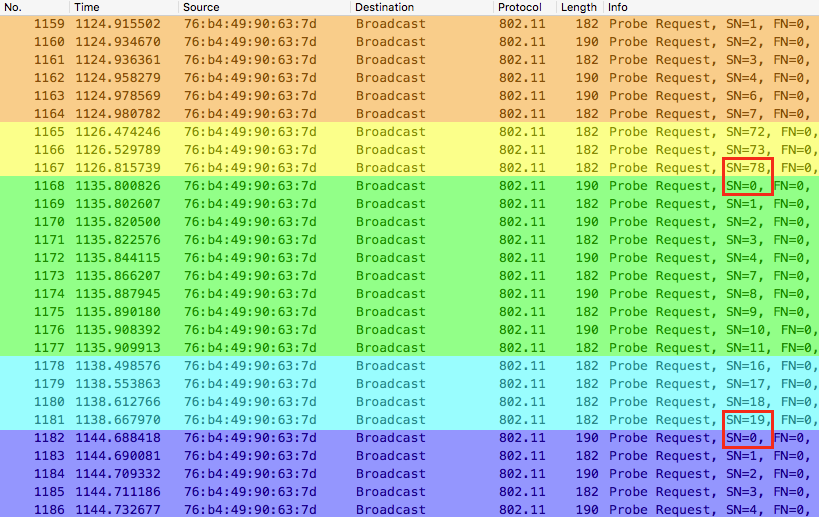
\includegraphics[width=\textwidth]{./img/result/randomization/ipad-mini}
	\end{table}

	% the SN
	\autoref{fig:ipad-random} depicts several examples of captured probe request packets from iPad mini, which were captured by Wireshark. The column represents, from left to right, the number of captured packet, the time of capture since beginning of capture (in second), the source address (\ac{MAC} address), the destination address, the communication protocol, packet length, and packet information.
	
	As we can see in~\autoref{fig:ipad-random}, the iPad mini reset the Sequence Number (\ac{SN}) after broadcasting two bursts of probe request. We can see in~\autoref{fig:ipad-random} that each burst, with nearly identical timestamp, is grouped in color. The red boxes mark the \ac{SN} reset, which mark a transition of \ac{SN} from 78 to 0, and 19 to 0.


	\subsection{Nexus 5X} % (fold)
	\label{sub:lg_nexus_5x}
	% when does the random mac appear?
	As opposed to iPad mini, Nexus 5X only sent out randomized \ac{MAC} address when the screen was off. When Nexus 5X woke up from sleep, it would immediately send out 4 or 10 probe request packets with real \ac{MAC} address. When Nexus 5X screen went off, Nexus 5X firstly sent out random \ac{MAC} address in every 2 to 10 seconds. Normally, Nexus 5X broadcast a burst of probe request packets roughly in each 60 seconds.

	Unlike iPad mini, Nexus 5X changed the \ac{MAC} address in each burst of probe request packets, as depicted in~\autoref{fig:nexus-random}. However, the first three octets were always the same and only the last three octets were changed. We can see that \verb|da:a1:19| appears in multiple bursts in~\autoref{fig:nexus-random} with different last three octets, \verb|ce:47:5f|, \verb|00:3f:25|, and \verb|b5:51:2c|, respectively.
	
	\begin{table}[h]
		\centering
		\caption[An example of captured probe requests from Nexus 5X.]{An example of captured probe requests from Nexus 5X in Wireshark. The colors mark out different bursts of probe request packets. The original \ac{MAC} address is indicated by cyan color in the last burst.}
		\label{fig:nexus-random}
		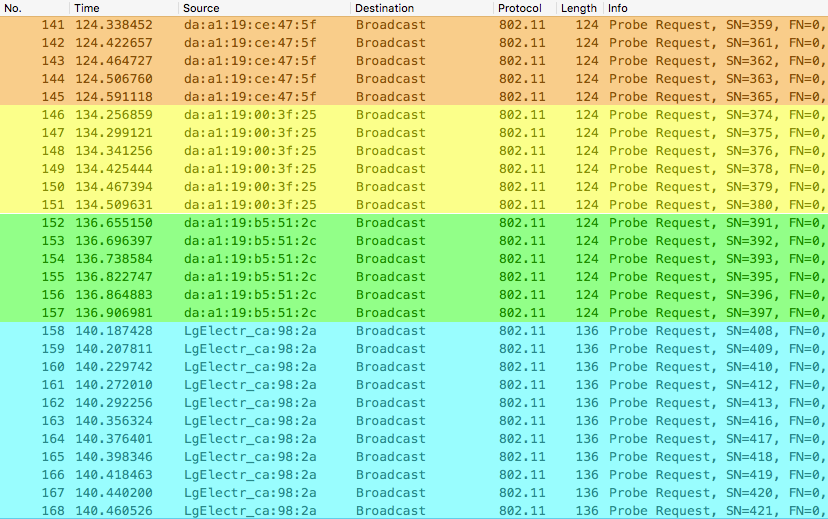
\includegraphics[width=\textwidth]{./img/result/randomization/nexus-5x}
	\end{table}	

	% the SN
	\autoref{fig:nexus-random}~depicts an example of captured probe request packets from Nexus 5X in the same format as~\autoref{fig:ipad-random}. There are four bursts of probe request packets marked in different colors. Three of the bursts are random \ac{MAC} address, while the last burst, marked in blue color, is the Nexus 5X original \ac{MAC} address.

	As we can see from~\autoref{fig:nexus-random}, the last probe request packet of a burst has a close \ac{SN} to the first packet of the next burst, although it is not sequential. We observed no obvious pattern in \ac{SN} change during the experiment.

	\subsection{Review} % (fold)
	\label{sub:review}
	% \added{
		Based on our findings in \ac{MAC} address randomization investigation, we can minimize the side-effect of \ac{MAC} address randomization by using one minute cycle length in data collection.
	% }
	This means we record the ambient noise and capture time-lapse images within 1 minute time interval, while we capture probe request packets in 52 seconds followed by two times of \ac{AP} scanning (see~\autoref{sub:scanning}).


% maybe use this
% Use table of simulation about randomized mac address using different time window.

\section{Correlation between Crowd Count and Sensor Readings} % (fold)
\label{sec:crowd_count_correlation-result}
In this section, we present the result of data collection using 1 minute cycle length, which consist of probe request packet capture, \ac{AP} scan, ambient noise recording, and time-lapse images capture (see~\autoref{fig:sensor-measurement}). As for the ground truth estimation, we used head count of time-lapse images and device count in unique \ac{MAC} address in probe request. The results indicate whether smartphone sensor readings can be an approach to estimate the level of social density or crowd count.

% when
We collected the data from Wednesday, October 26\textsuperscript{th} 2016, to Saturday, October 29\textsuperscript{th} 2016. The timing of data collection is shown in~\autoref{tab:location-summary}. During the data collection, we observed no special events in which the social density level are much higher than the normal condition, especially in public places, such as Grote Markt and Paddepoel shopping center.

% assumption
In manual head counting, a person might appear more than once, i.e., the person was captured in multiple GoPro cameras, because we took time-lapse images and some people were actively moving. We make sure that the people who appear several times in different images are counted exactly once. Furthermore, sometimes we captured vehicles with very limited visual appearance of the people inside. We assume that there are a person in a car and five people in a bus. We present some examples of time-lapse images in~\autoref{ch:appendix-time-lapse-images}.

\begin{figure}[h]
	\begin{adjustwidth}{-2cm}{}
	\centering
	\subfloat[head count]{
		\label{fig:population-head-count}{
			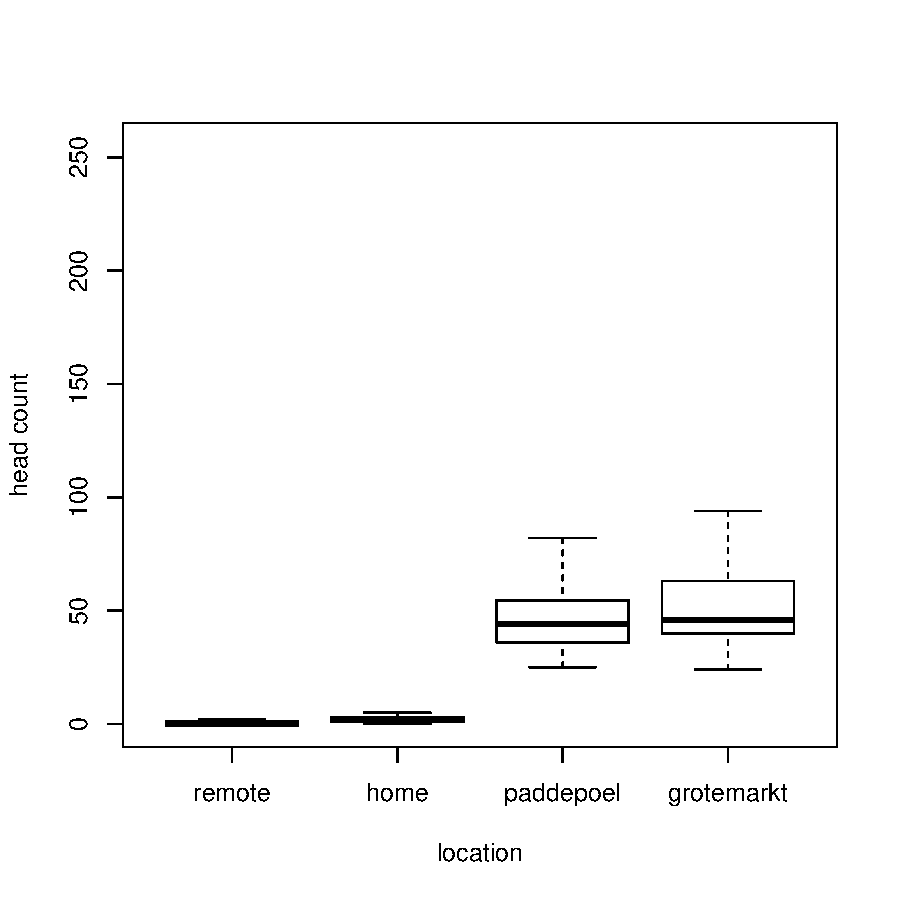
\includegraphics[width=0.65\textwidth]{./img/result/boxplot-hc-small}
		}
	}
	\subfloat[device count]{
		\label{fig:population-device-count}{
			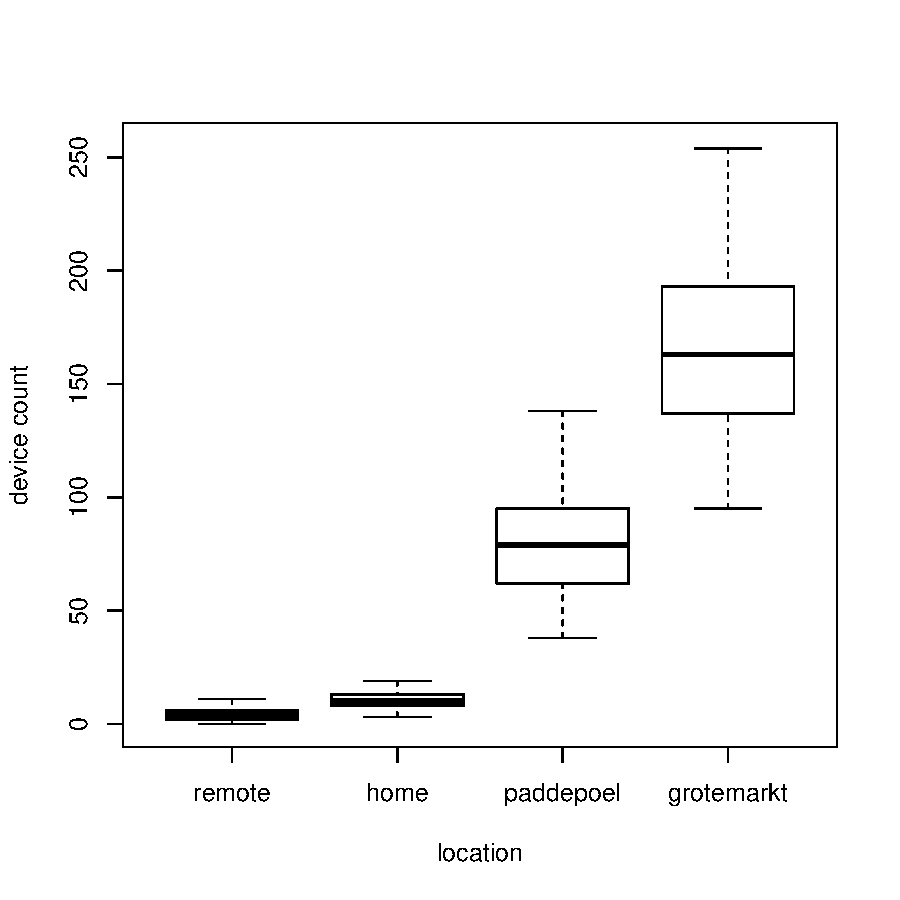
\includegraphics[width=0.65\textwidth]{./img/result/boxplot-dc-small}
		}
	}
	\end{adjustwidth}
	\caption[A box plot of the population]{A box plot showing the population of estimated social density in each location by head count (\ref{fig:population-head-count}) and device count (\ref{fig:population-device-count}).}
	\label{fig:total-population}
\end{figure}

We present the important results of the experiment, such as the variation of the social density level, example of ambient noise recording, correlation of \ac{AP} count and sensor readings, the effect of scanning time, and all parameters used for analysis. The appendices present the detailed results, such as the sensor readings both in scatter plot and line chart (\autoref{ch:appendix-sensor-readings}), example of time-lapse images for each location (\autoref{ch:appendix-time-lapse-images}), and ambient noise recording (\autoref{ch:appendix-ambient-noise}).

\autoref{fig:total-population}~depicts the variation of the estimated social density level in each location, e.g., the lowest value, the first quartile, the median, the upper quartile, and the maximum value. The value are estimated by two approximation, namely head count (\ref{fig:population-head-count}) and device count (\ref{fig:population-device-count}).

As we can see in~\autoref{fig:total-population}, the maximum value of the device count based estimation is higher than the head count based estimation. For instance, in Grote Markt, the maximum value of device count is 288, while the maximum value of head count is 115. However, both estimations are showing the same trend, which says that Grote Markt has the highest social density level and remote area has the lowest social density level.

% device count
%    LOC Min  Q1 Med  Q3 Max
% 1:   r   0   2   4   6  11
% 2:   h   3   8  10  13  46
% 3:   p  38  62  79  95 150
% 4:   g  95 137 163 193 288

% head count
%    LOC Min Q1 Med   Q3 Max
% 1:   r   0  0   0  1.0   4
% 2:   h   0  1   2  3.0   5
% 3:   p  25 36  44 54.5  95
% 4:   g  24 40  46 63.0 115











	\subsection{Ambient Noise Recordings} % (fold)
	\label{sub:ambient_noise_recordings}
	As an example of ambient noise recording, \autoref{tab:ambient-noise-average-day4} and \autoref{fig:audio-result-day4} show the result of ambient noise recording in day 4, when more crowds were present than any other days. We measure the ambient noise in decibels (dB). In this unit, the closer the value to zero, the louder the sound (noise). We take two measures of ambient noise to characterize the surrounding, namely Peak Level (\ac{PKLV}), which is the highest value of a total waveform, and Root Mean Square (\ac{RMS}), which is the effective value or the mean of an audio recording. \ac{PKLV} and \ac{RMS} are positively correlated but \ac{RMS} is more stable than \ac{PKLV}.

	\begin{table}[H]
	\centering
	\caption[]
	{The average of RMS and PKLV of ambient noise recording in day 4.}
	\label{tab:ambient-noise-average-day4}
	\begin{tabular}{lll}
	\toprule
	            & \ac{RMS} (dB) & \ac{PKLV} (dB) \\ \midrule
	Remote area &  -47.74           &  -26.90    \\
	Home        &  -39.39         & -12.84       \\
	Paddepoel   & -26.54          &  -3.39       \\
	Grote markt & -36.29             & -5.87     \\ \bottomrule
	\end{tabular}
	\end{table}

	\begin{figure}[H]
		% \centering
		\subfloat[peak level]{
			\label{fig:peak-level-day4}{
				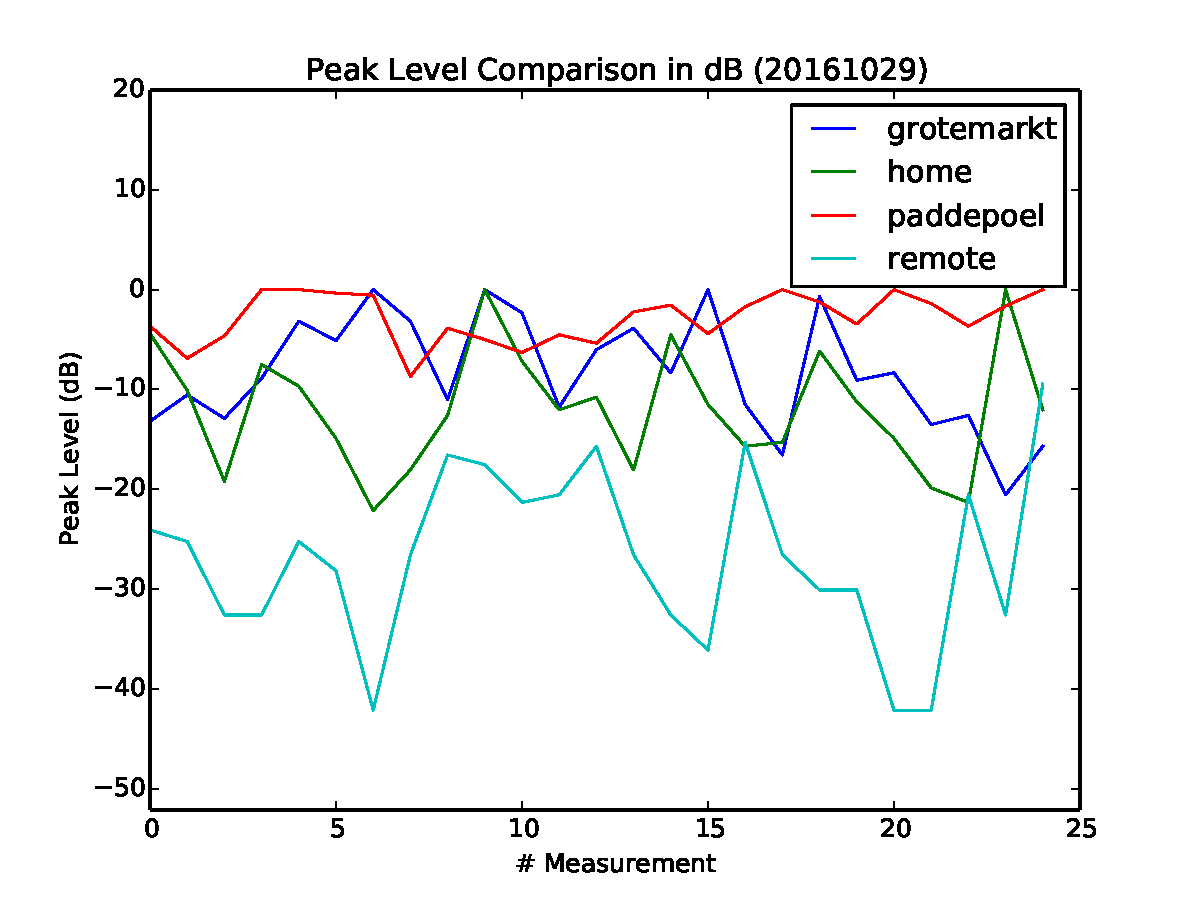
\includegraphics[width=0.8\textwidth]{./img/result/sound/peak-level-comparison-20161029}
			}
		}\\
		\subfloat[root mean square]{
			\label{fig:rms-day4}{
				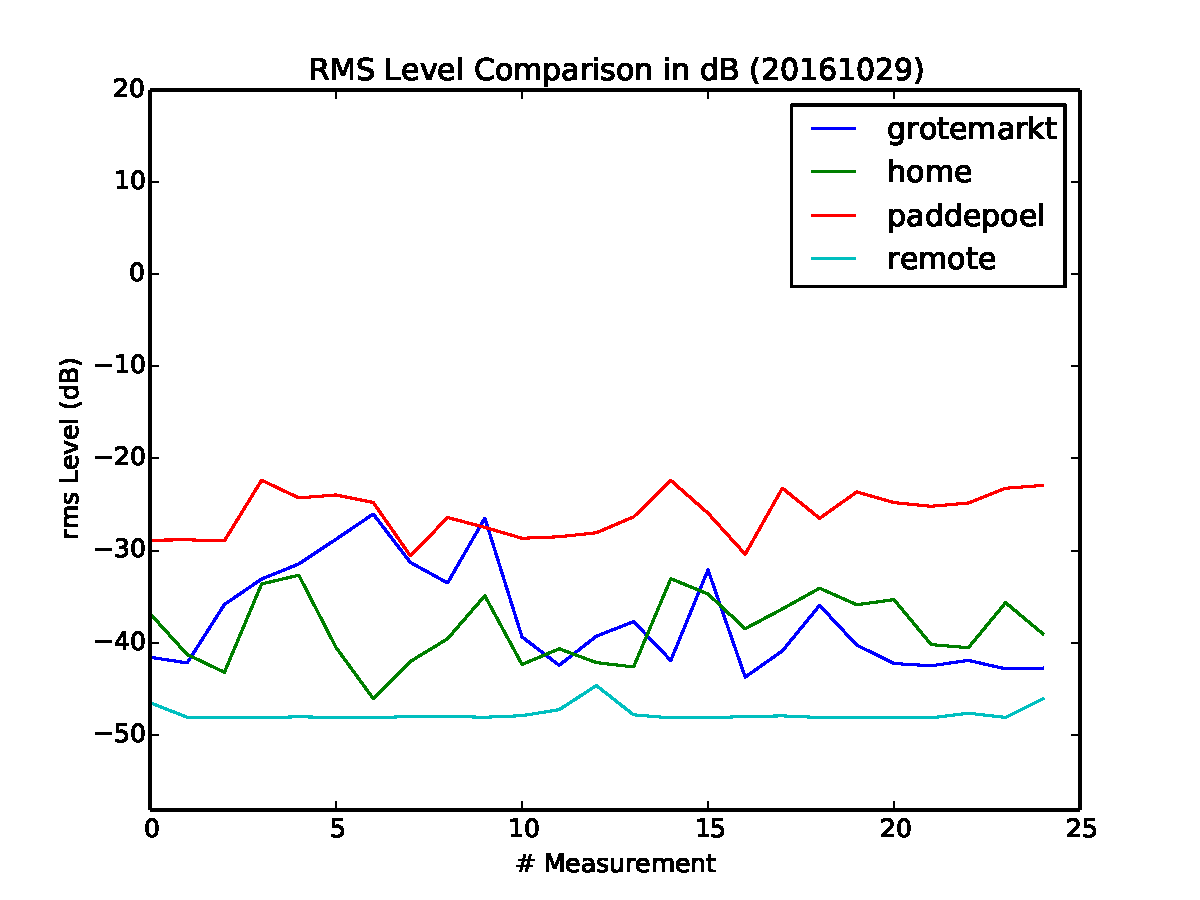
\includegraphics[width=0.8\textwidth]{./img/result/sound/rms-level-comparison20161029}
			}
		}
		\caption[Line chart of ambient noise at day 4]{Line chart showing the peak level (\ref{fig:peak-level-day4}) and root-mean-square (\ref{fig:rms-day4}) of the ambient noise recording in each cycle at day 4.}
	\label{fig:audio-result-day4}
	\end{figure}

	As we can see in the average value (\autoref{tab:ambient-noise-average-day4}) or line chart (\autoref{fig:audio-result-day4}), more crowded place has higher ambient noise value. We see that remote area is the quietest location, with -47.74 dB of average \ac{RMS}, while Paddepoel is the noisiest location, with -26.54 dB of average \ac{RMS}. As for the line chart, we can see more overlaps in \ac{PKLV} (\autoref{fig:peak-level-day4}) than in \ac{RMS} (\autoref{fig:rms-day4}). The \ac{RMS} of remote area is stable near -50.00 dB. We can also see the same trends for the rest of the ambient noise recordings, although some overlaps are present, as shown in~\autoref{ch:appendix-ambient-noise}.


	% \subsubsection{Speaker Count Extraction} % (fold)
	% \label{ssub:probe_request_based_estimation}
	% In~\autoref{sec:line_charts}, we present the result of smartphone sensor readings that displays the estimated speaker count from ambient noise recording, extracted using unsupervised machine learning method by Xu, et al,~\cite{thesis067}. However, the result is not satisfying as the speaker count estimation is mostly yielding zero speaker count, even in the most crowded location. When we listened to the audio recording, sometimes human voice is present but not apparent and clear.

	% To test the accuracy of unsupervised speaker count estimation from Xu, et al,~\cite{thesis067}, we apply the algorithm to audio recordings in which the speaker voice is apparent and clear. We select different audio recordings that have diverse speaker count, ranging from single speaker, as in a speech or monologue, two speakers, as in duets or interview, and five speakers, as in a cappella.

	% We tune two parameters in the speaker count algorithm, namely ${\theta}_{s}$ and ${\theta}_{d}$, using recommended configuration in their implementation of the algorithm\footnote{\url{https://github.com/lendlice/crowdpp}}. The ${\theta}_{s}$ parameter refers to the confidence level that we can identify the same speaker, while ${\theta}_{d}$ is about new speaker. \autoref{tab:speaker-count-result} summarizes the result.

	% \begin{table}[h]
	% \begin{adjustwidth}{-2cm}{}
	% \centering
	% \caption{Speaker count result}
	% \label{tab:speaker-count-result}
	% \begin{tabular}{l|l|llllll}
	% \toprule
	% \multirow{2}{*}{Description} & \multirow{2}{*}{\specialcell{Total\\Speaker(s)}} & \multicolumn{6}{c}{Detected Speaker(s) (${\theta}_{s},{\theta}_{d}$)} \\
	%                              &                                & (13, 18) & (14, 24) & (15.6, 21.6) & (16, 21) & (17, 22) & (18, 25) \\ \midrule
	% speech                     & 1 & 11 & 5 & 6 & 7 & 6 & 5 \\
	% monologue                    & 1 & 5 & 4 & 5 & 5 & 5 & 3 \\
	% duets                        & 2 & 1 & 1 & 1 & 1 & 1 & 1 \\
	% interview     			 & 2 & 5 & 5 & 5 & 5 & 5 & 5 \\
	% a cappella                   & 5 & 5 & 4 & 4 & 4 & 4 & 4 \\
	% \bottomrule 
	% \end{tabular}
	% \end{adjustwidth}
	% \end{table}

	% We can see from~\autoref{tab:speaker-count-result} that the speaker estimation is not accurate. The only accurate estimation is done using 13 and 18 as the ${\theta}_{s}$ and ${\theta}_{d}$, respectively, but it only applies to a cappella recording with five speakers. The estimation gives stable result for duets and interview recording along different combination of ${\theta}_{s}$ and ${\theta}_{d}$, although it is not correct. 







	\subsection{AP and Social Density Correlation} % (fold)
	\label{sub:ap_and_social_density_correlation}
	We are particularly interested in seeing the trend and correlation of WiFi \ac{AP} count and social density level, estimated by head count and device count. We draw a scatter plot of \ac{AP} count vs device count and \ac{AP} count vs head count separately, as well as device count vs head count to see the correlation of the two social density estimation. The plots are shown in~\autoref{fig:scatter-dc-ap}, \autoref{fig:scatter-hc-ap}, and \autoref{fig:scatter-hc-dc}. We also present the line chart of the readings in~\autoref{ch:appendix-sensor-readings}.

	\autoref{fig:scatter-dc-ap} depicts the correlation of device count and \ac{AP} count. The data plotted in~\autoref{fig:scatter-dc-ap} come from all data from four days of experiments. The location is coded in color so that we can distinguish which data come from which location. The plots of the correlation separately in each day are also available in~\autoref{ch:appendix-sensor-readings}, shown in~\autoref{fig:ap-dc-scatterplot}.
	
	As we can see in~\autoref{fig:scatter-dc-ap} there is a positive trend that indicates both variables have a positive correlation. This means when the \ac{AP} count increases, the device count, which points to social density level, increases as well. The correlation coefficient $\rho$ is 0.877, indicating a strong correlation, and the $p$-value is below 0.05, indicating that the result is significant.
	% \added{
		Each location forms a distinguishable cluster, although some overlaps are present.
	% }
	The cluster of home and remote are close and the cluster of Paddepoel and Grote Markt are adjacent. However, there is a gap that separates home-remote cluster and Paddepoel-Grote markt cluster.

	% all result - device count
	\begin{figure}[h]
		\centering
		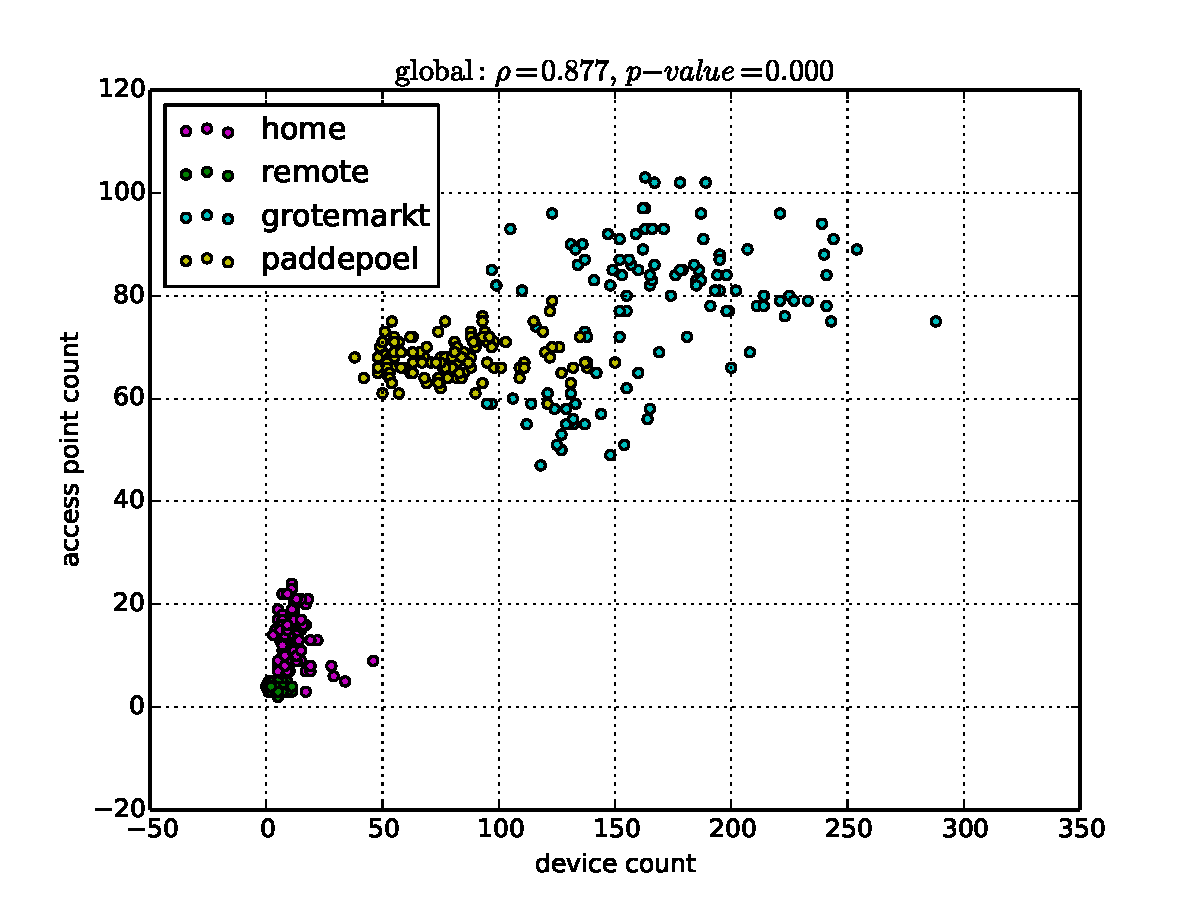
\includegraphics[width=0.8\textwidth]{./img/result/global-pr-vs-ap}
		\caption[Scatter plot of device and \ac{AP} count.]
		{Scatter plot showing the correlation between \textit{device count} and \textit{\ac{AP} count} of all collected data. The locations are marked in different color. The correlation coefficient is $\rho=0.877$.}
		\label{fig:scatter-dc-ap}
	\end{figure}

	\autoref{fig:scatter-hc-ap} portrays the correlation between head count and \ac{AP} count of data collected in four days of all location. \autoref{fig:scatter-hc-ap} uses the same color coding as~\autoref{fig:scatter-dc-ap} to distinguish the location. The plots showing the correlation in separate days are available in~\autoref{ch:appendix-sensor-readings}, shown in~\autoref{fig:ap-hc-scatterplot}.
	
	We can see similar trend in~\autoref{fig:scatter-hc-ap}. The correlation is strong, indicated by correlation coefficient $\rho = 0.877$, and significant, indicated by p-value which is below 0.05. However, the Grote Markt and Paddepoel clusters are overlapping each other. A gap between remote-home cluster and Grote Markt-Paddepoel cluster is also present.

	% all result - head count
	\begin{figure}[H]
		\centering
		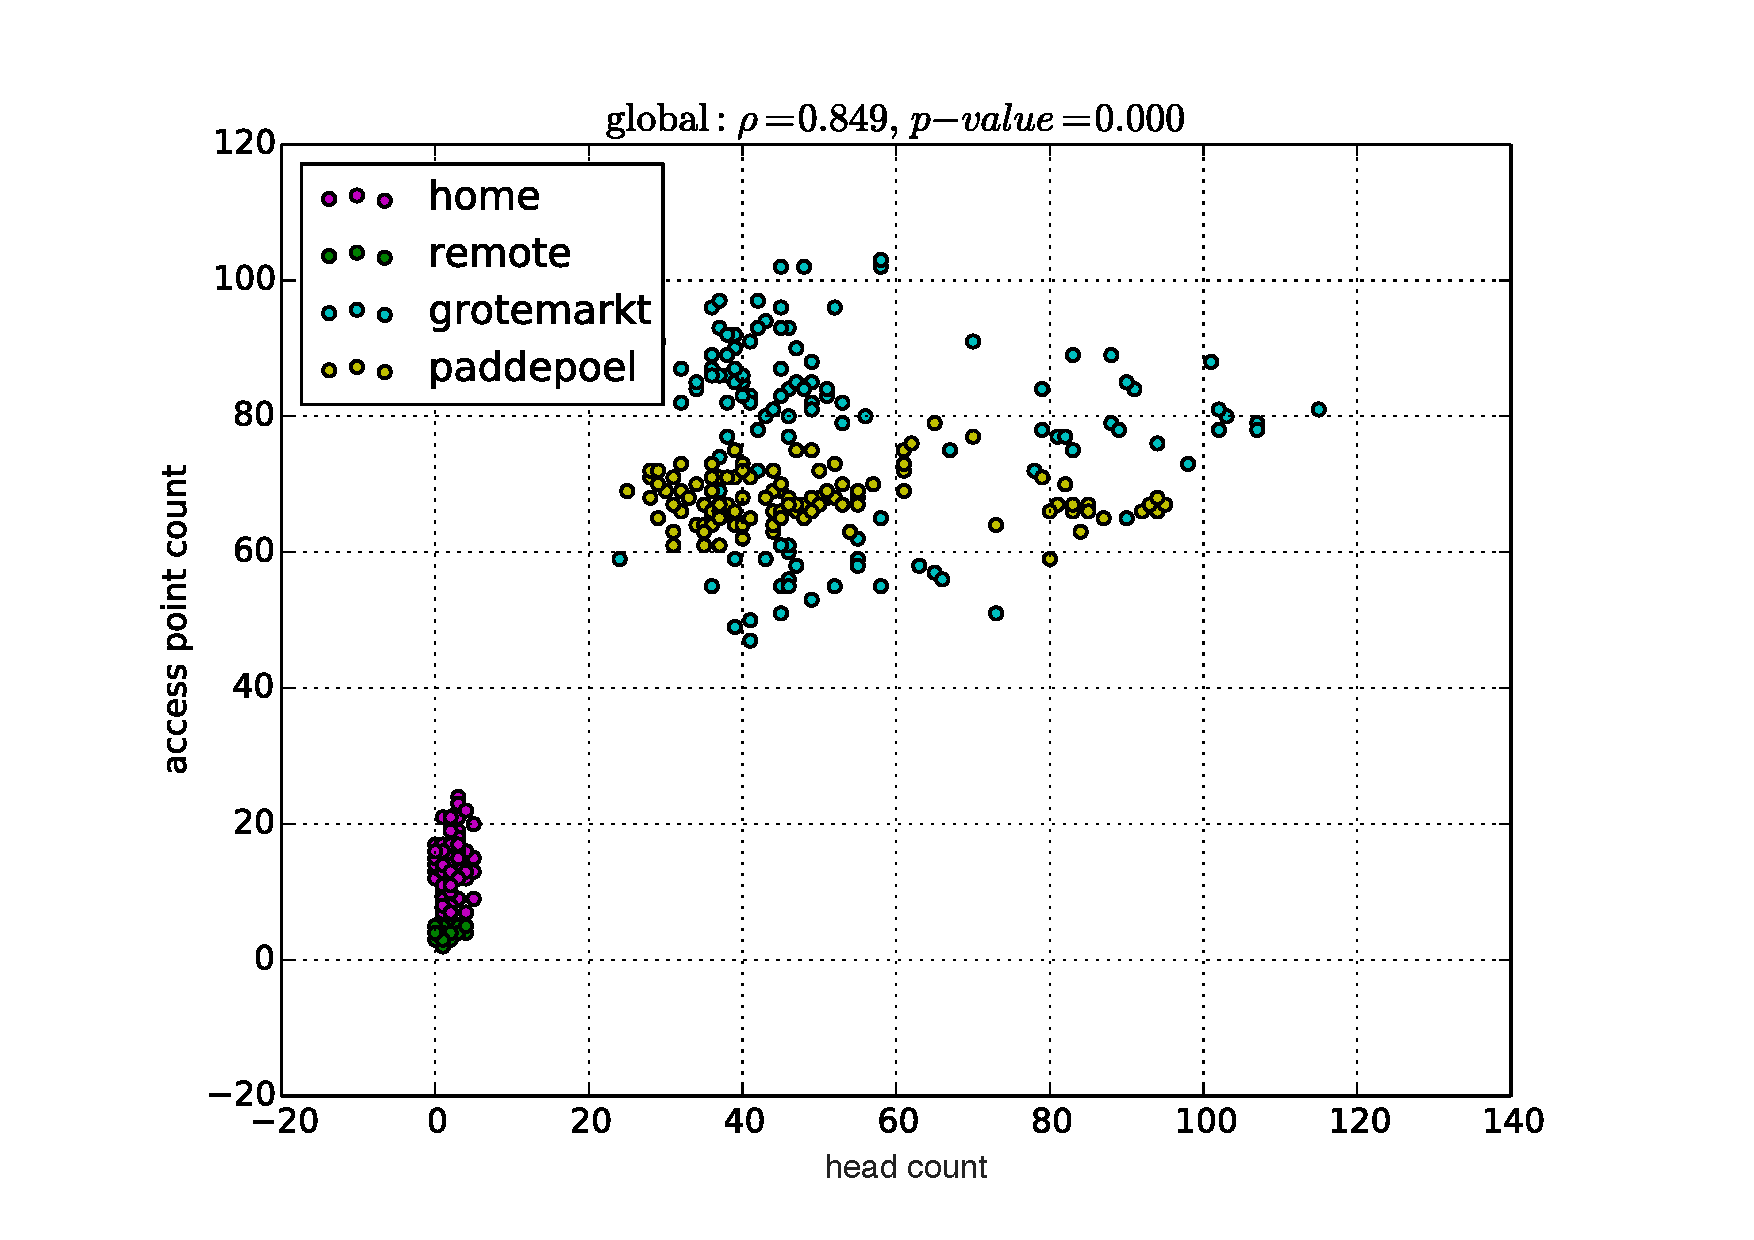
\includegraphics[width=0.8\textwidth]{./img/result/global-gt-vs-ap}
		\caption[Scatter plot of head and \ac{AP} count.]
		{Scatter plot showing the correlation between \textit{head count} and \textit{\ac{AP} count} of all collected data. The locations are marked in different color. The correlation coefficient is $\rho=0.849$.}
		\label{fig:scatter-hc-ap}
	\end{figure}

	\autoref{fig:scatter-hc-dc} shows the correlation of head count and device count of all collected data. The locations are coded in color as well. Head count and device count have a strong correlation, marked by the correlation coefficient $\rho$, which is 0.857. A gap between remote-home cluster and Grote Markt-Paddepoel cluster is also present, although it is narrower than the gap in \autoref{fig:scatter-dc-ap} and \autoref{fig:scatter-hc-ap}. \autoref{fig:hc-dc-scatterplot} in \autoref{ch:appendix-sensor-readings} presents the scatter plots showing the correlation of head count and device count in each day of the experiment.

	% all result - device count vs head count
	\begin{figure}[H]
		\centering
		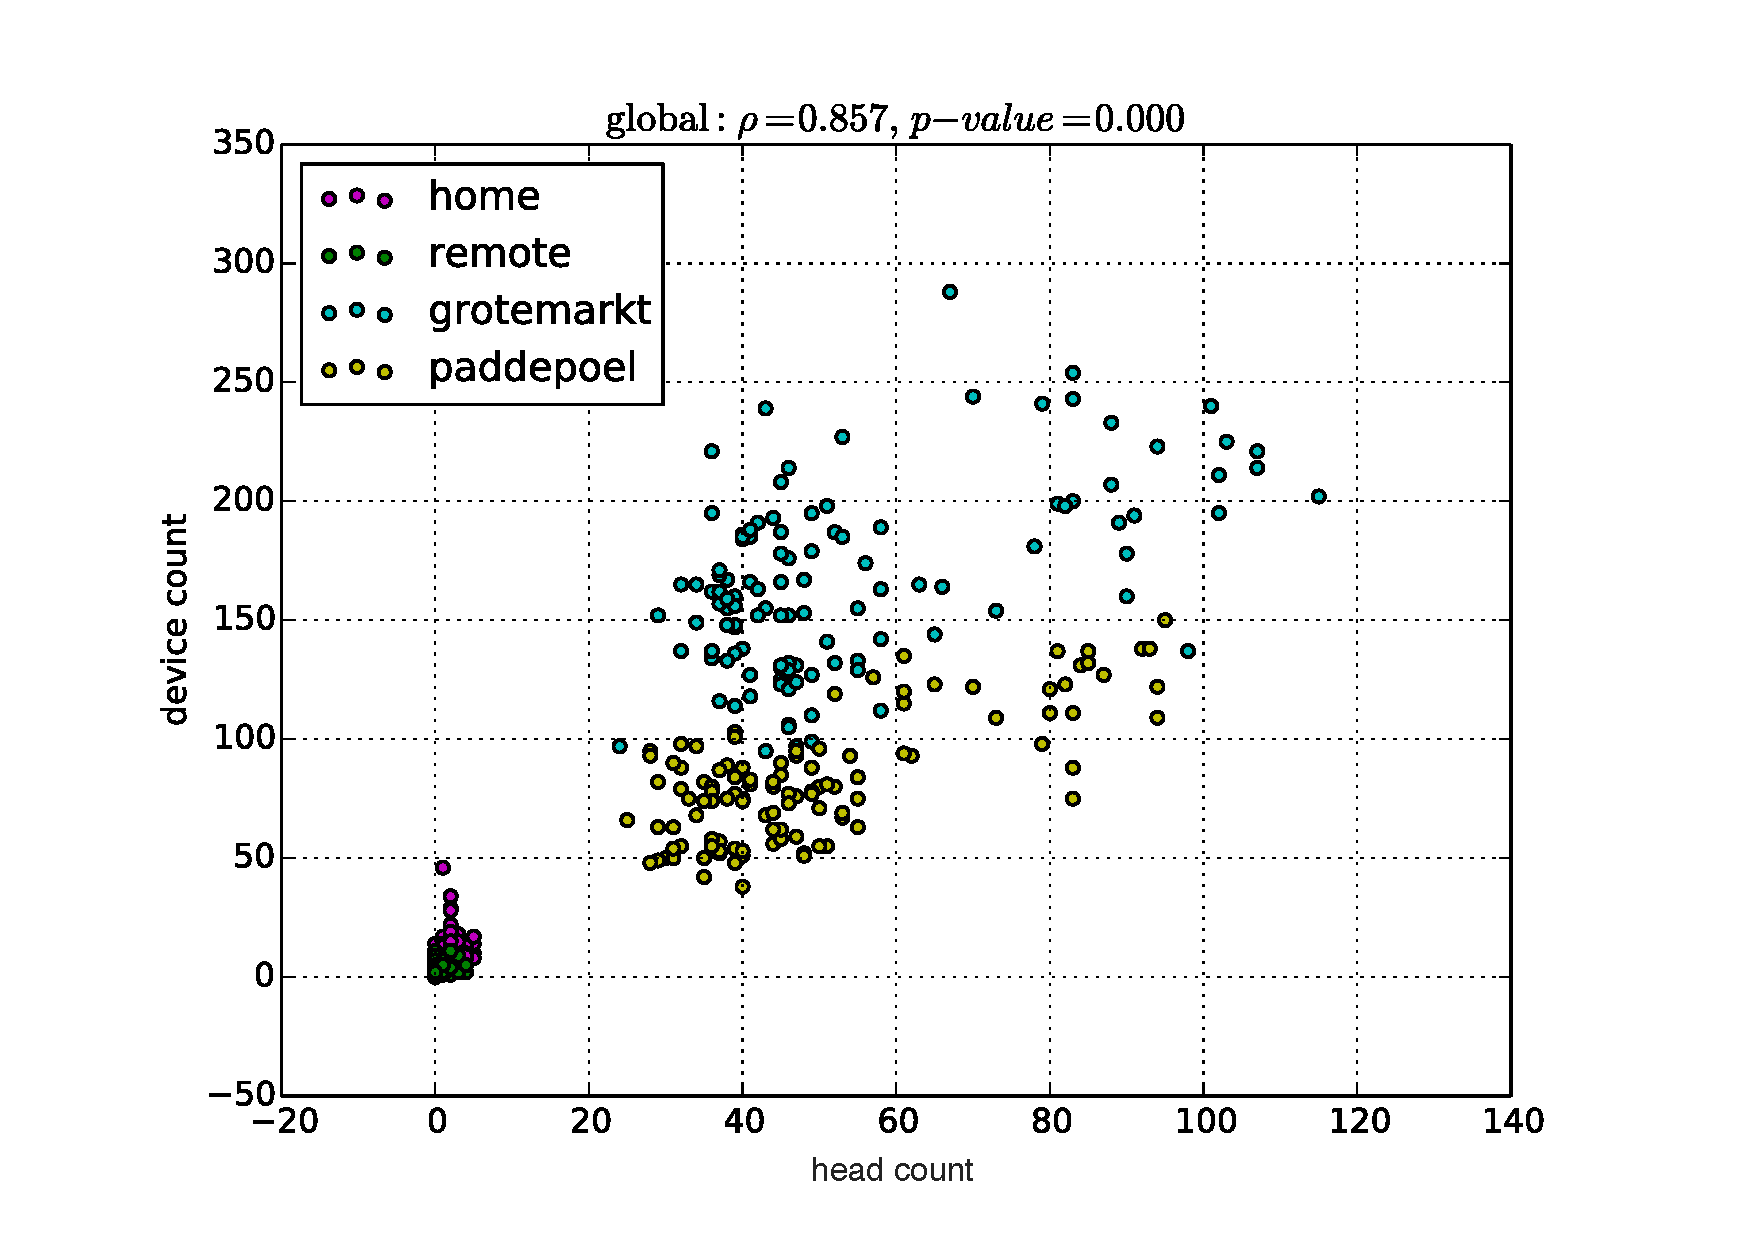
\includegraphics[width=0.8\textwidth]{./img/result/global-gt-vs-pr}
		\caption[Scatter plot of head and device count.]
		{Scatter plot showing the correlation between \textit{head count} and \textit{device count} of all collected data. The locations are marked in different color. The correlation coefficient is $\rho=0.857$.}
		\label{fig:scatter-hc-dc}
	\end{figure}

	As we can see in three scatter plots (\autoref{fig:scatter-dc-ap}, \autoref{fig:scatter-hc-ap}, and \autoref{fig:scatter-hc-dc}), \ac{AP} and social density level from both head count and device count have a positive correlation. The correlation is strong, which is roughly 0.8 with p-value less than 0.05. 






	\subsection{Effect of Scanning Time} % (fold)
	\label{sub:effect_of_scanning_time}
	We performed four experiments on Sunday, October 30\textsuperscript{th} 2016, to investigate the effect of scanning time to the \ac{AP} count and social density correlation. We collected the data for 45 minutes, consisting WiFi and audio data, in four different scanning time, namely
	\begin{enumerate*}[label={\alph*)},font={\color{red!50!black}\bfseries}]
	  \item 09:00,
	  \item 12:00,
	  \item 15:00,
	  \item and 18:00
	\end{enumerate*}.
	
	\autoref{fig:time-effect} shows the WiFi scanning result in four separate line charts. Each chart depicts the result of a certain scanning time. The blue lines, which depict the \ac{AP} count, fluctuate stably around 100, while the green lines, which represent the device count, have a big variance. As we can see in~\autoref{fig:grotemarkt-0900}, the green line is fluctuating below the blue line, indicating there were less device than available \ac{AP} count. However, in~\autoref{fig:grotemarkt-1200}, \autoref{fig:grotemarkt-1500}, and \autoref{fig:grotemarkt-1800}, the condition changes. The green lines surpass the blue lines, which indicates that the number of device was increased. \autoref{fig:grotemarkt-1500} shows an increasing trend of device count, while \autoref{fig:grotemarkt-1800} shows a decreasing trend.

	\begin{figure}[H]
		\centering
		\begin{adjustwidth}{-3cm}{}
		\subfloat[09:00h]{
		  \label{fig:grotemarkt-0900}{
		    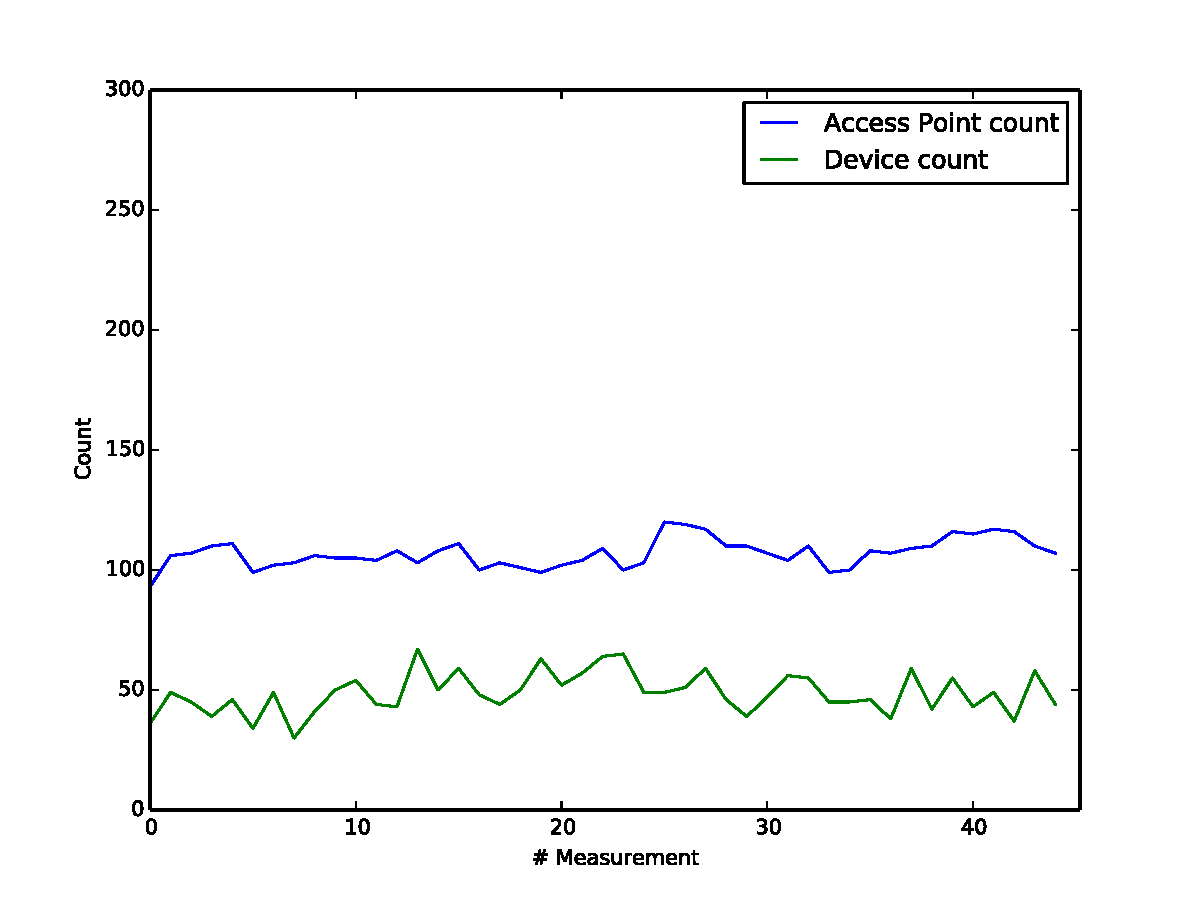
\includegraphics[width=0.7\textwidth]{./img/result/time/grotemarkt-0900}
		  }
		}
		\subfloat[12:00h]{
		  \label{fig:grotemarkt-1200}{
		    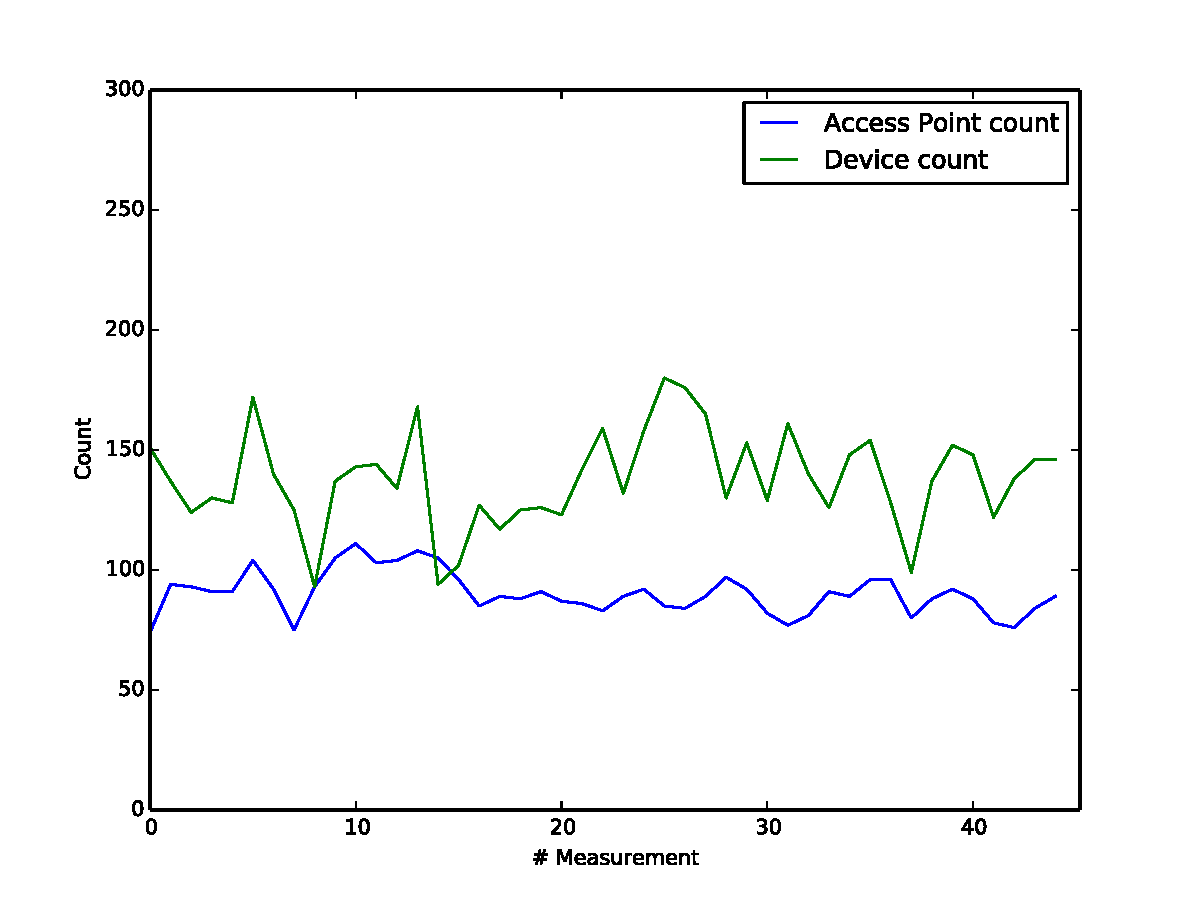
\includegraphics[width=0.7\textwidth]{./img/result/time/grotemarkt-1200}
		  }
		}\\
		\subfloat[15:00h]{
		  \label{fig:grotemarkt-1500}{
		    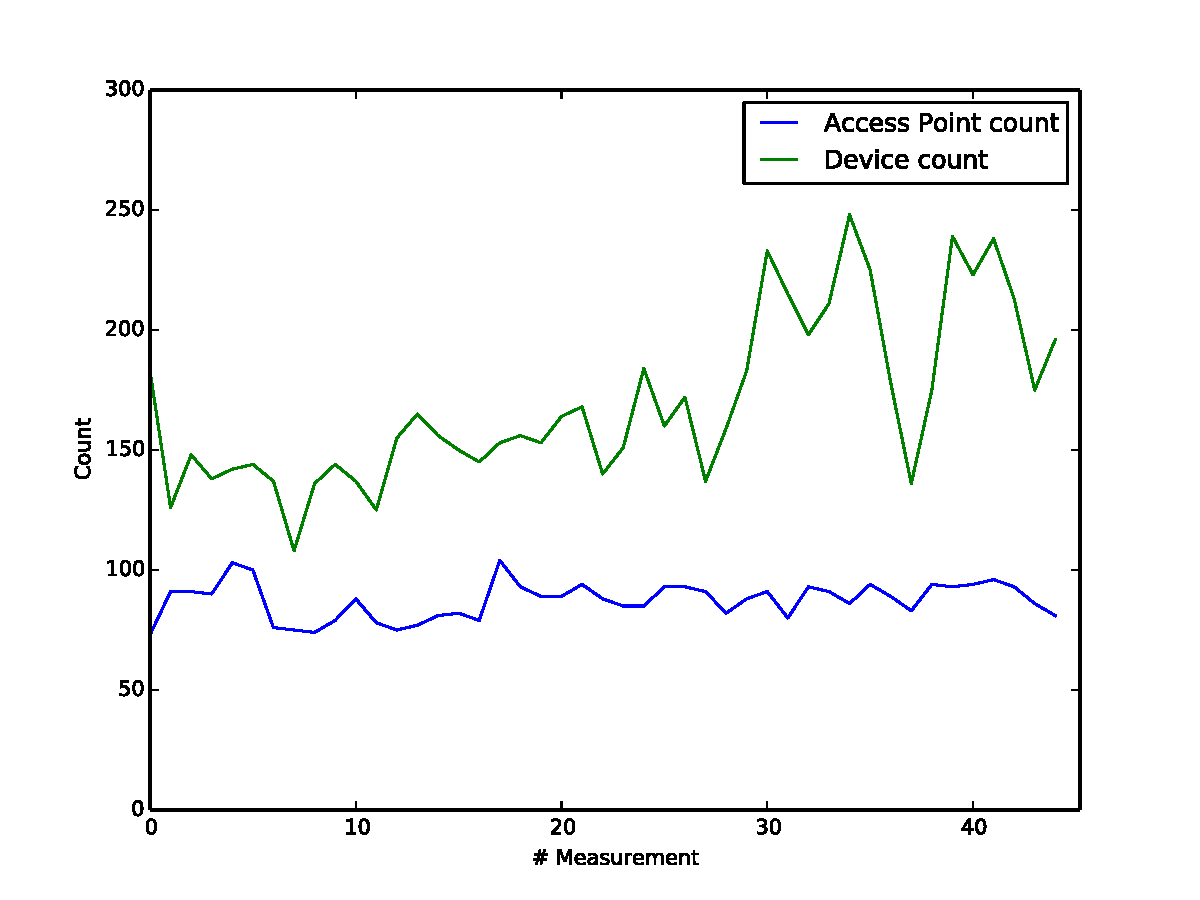
\includegraphics[width=0.7\textwidth]{./img/result/time/grotemarkt-1500}
		  }
		}
		\subfloat[18:00h]{
		  \label{fig:grotemarkt-1800}{
		    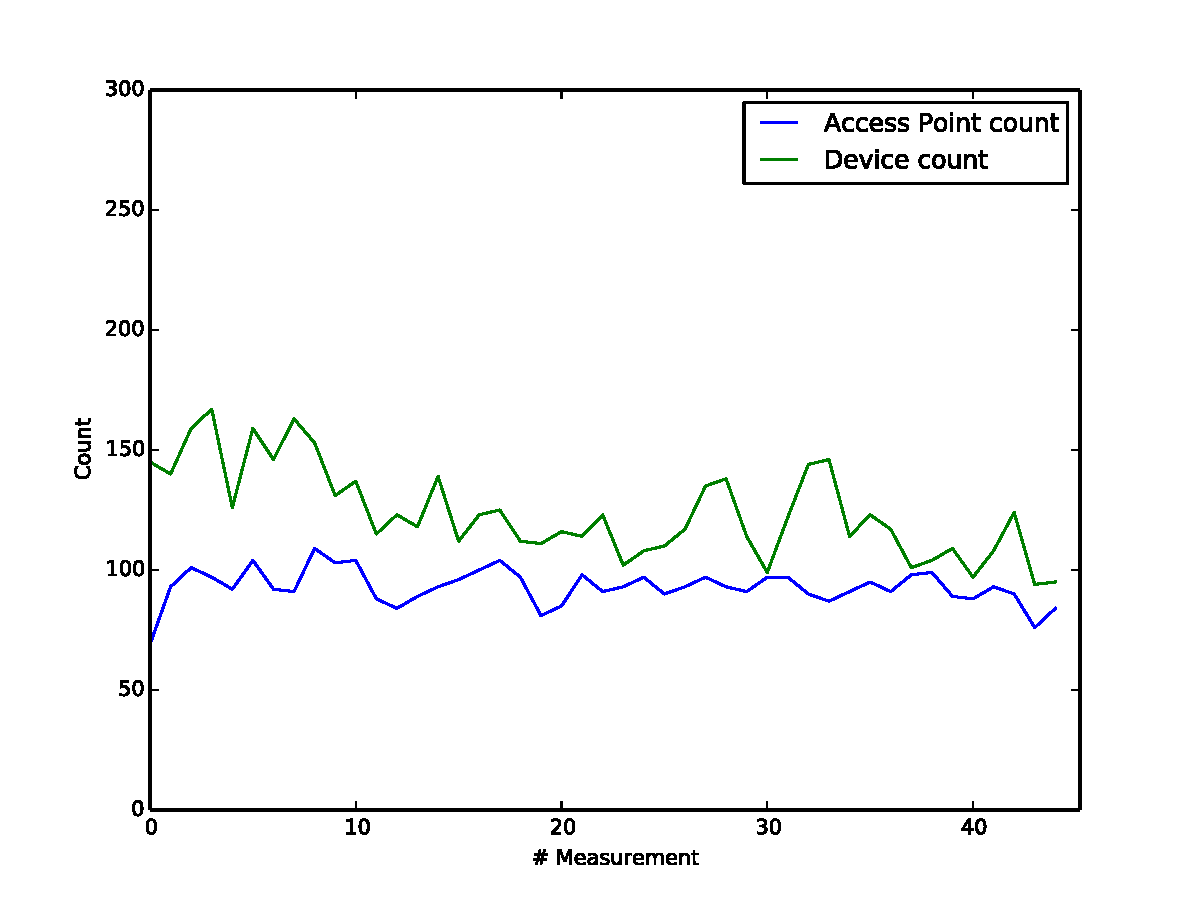
\includegraphics[width=0.7\textwidth]{./img/result/time/grotemarkt-1800}
		  }
		}
		\caption[Line charts of ambient noise on October 30, 2016.]
		{Line charts showing the \ac{AP} count (blue) and device count (green) in different data collection time at Grote Markt, Groningen, on October 30, 2016.}
		\label{fig:time-effect}
		\end{adjustwidth}
	\end{figure}

	% \added{
	Moreover, we present the ambient noise recording of the Sunday, October 30\textsuperscript{th} 2016 experiment in~\autoref{tab:ambient-noise-timely} and \autoref{fig:audio-result-timely}. If we look at the line charts (\autoref{fig:audio-result-timely}), the lines are mostly overlapping each other, making it difficult to distinguish the noise characteristics of each scanning time. However, the ambient noise summary in~\autoref{tab:ambient-noise-timely} presents more understandable characteristics. We see that, in \ac{PKLV}, the noise is increasing from 09:00h, peaking at 15:00h, and going back down at 18:00h. The ambient noise recordings are correlated with the WiFi scanning results presented in~\autoref{fig:time-effect}.

	\begin{table}[h]
	\centering
	\caption[The average of RMS and PKLV of ambient noise in four scanning time.]
	{The average of root-mean-square and peak level of ambient noise recording in four different scanning time.}
	\label{tab:ambient-noise-timely}
	\begin{tabular}{lll}
	\toprule
	       & \ac{RMS} (dB) & \ac{PKLV} (dB) \\ \midrule
	09:00h & -40.51        & -14.95          \\
	12:00h & -40.91        & -13.08          \\
	15:00h & -37.53        & -8.90           \\
	18:00h & -40.62        & -12.41          \\ \bottomrule
	\end{tabular}
	\end{table}

	\begin{figure}[h]
		% \centering
		\begin{adjustwidth}{-1cm}{}
		\subfloat[peak level]{
			\label{fig:peak-level-timely}{
				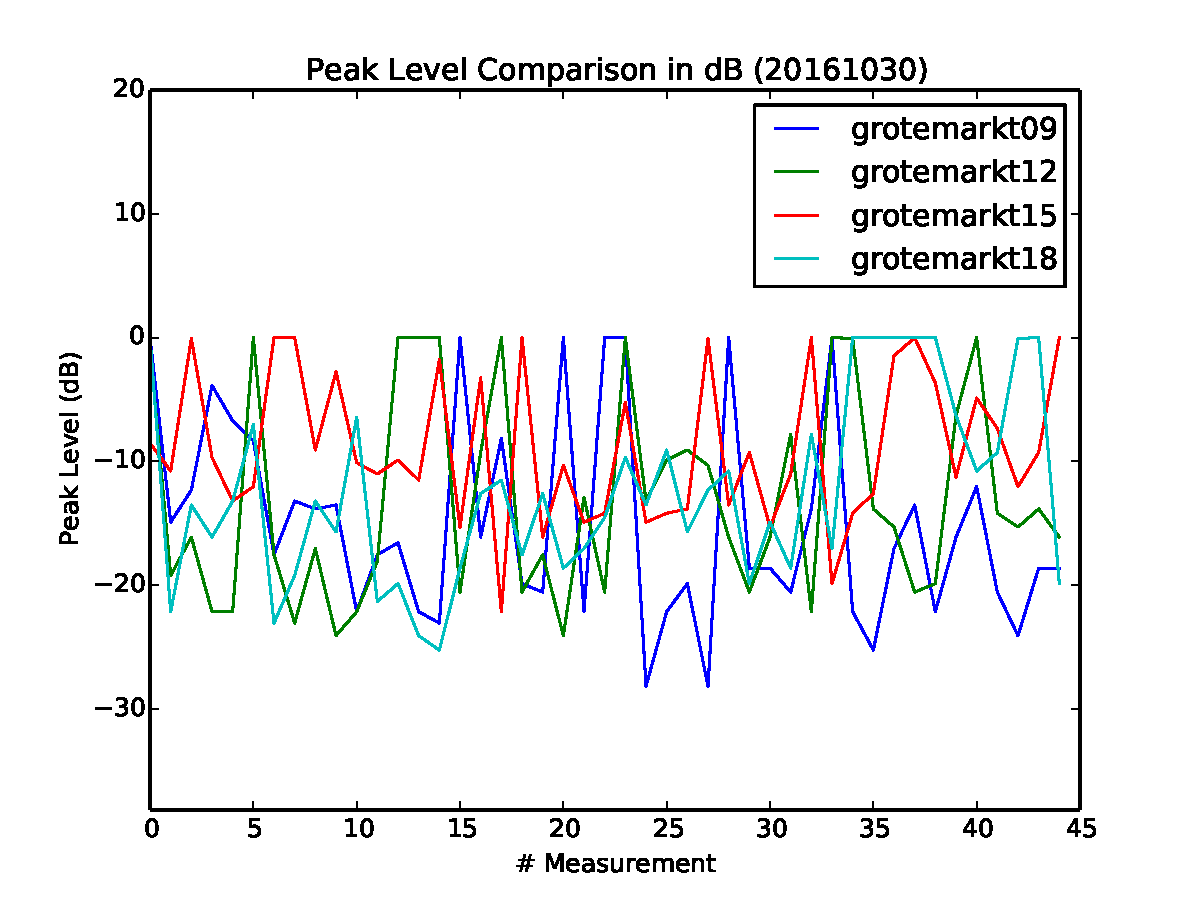
\includegraphics[width=0.6\textwidth]{./img/result/time/peak-level-comparison}
			}
		}
		\subfloat[root mean square]{
			\label{fig:rms-timely}{
				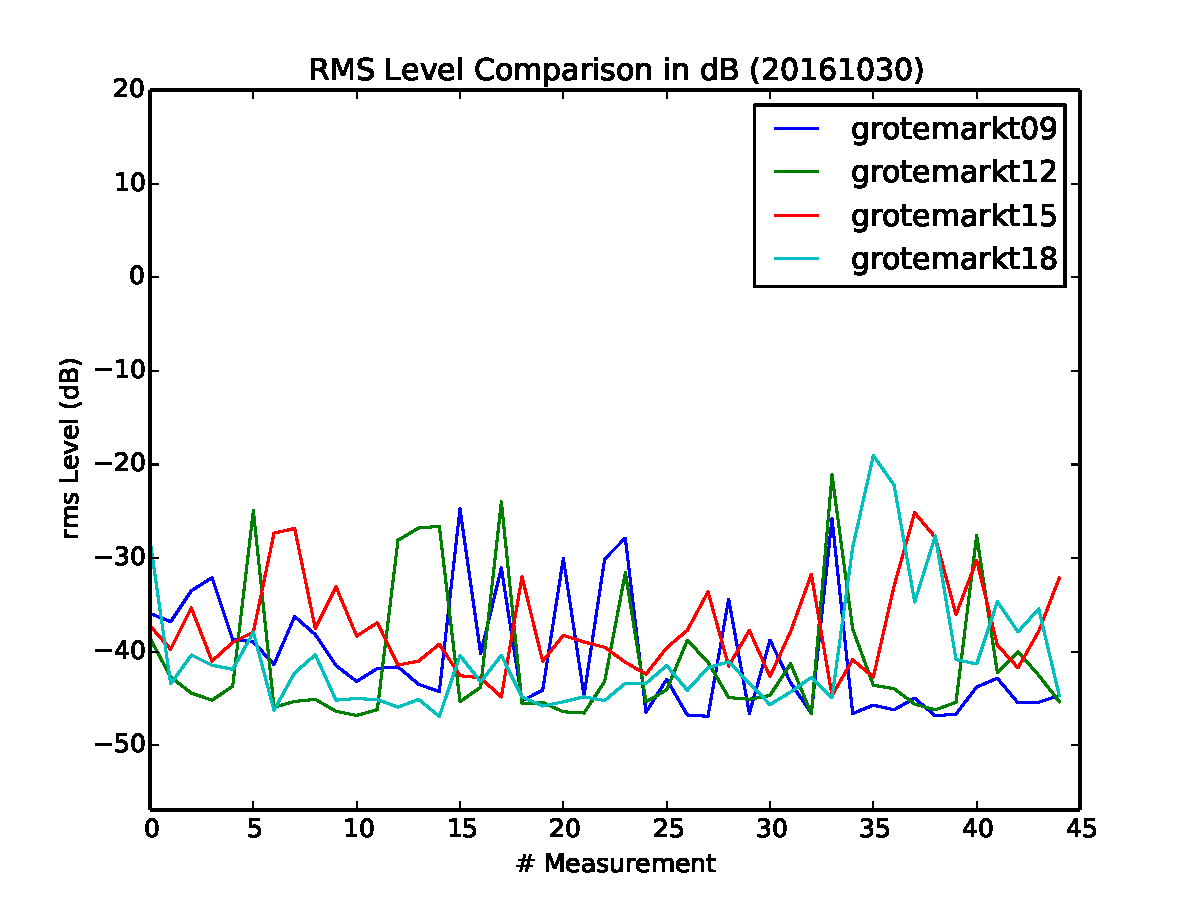
\includegraphics[width=0.6\textwidth]{./img/result/time/rms-level-comparison}
			}
		}
		\caption[Ambient noise in different scanning time.]
		{Line charts showing the peak level (\ref{fig:peak-level-timely}) and root-mean-square (\ref{fig:rms-timely}) of the ambient noise recording in four diffent scanning time.}
		\label{fig:audio-result-timely}
		\end{adjustwidth}
	\end{figure}
	% }



	\subsection{All Result} % (fold)
	\label{sub:all_result}
	\autoref{fig:scatterplot-matrix} shows all data collected in four days of experiments in a scatter plot matrix. In the lower left part are the scatter plots of each parameter correlation along with the Lowess curve fitted to the data. In the upper part are the correlation coefficient and the p-value. Along the diagonal are the histograms and the labels of each parameter.

	There are eight parameters extracted from all datasets of four days experiment. The \ac{AP}, \ac{RSSI}, \ac{DC}, and \ac{SNR} parameters are from WiFi based readings. \ac{AP} is the count of available \ac{AP} that a smartphone can get, while \ac{RSSI} is the average of the signal strength of the \ac{AP}. \ac{DC} is the device count, based on unique \ac{MAC} address, and \ac{SNR} is the average of signal-to-noise ratio of the captured probe request packets. \ac{SC}, \ac{RMS}, and \ac{PKLV} are from recorded ambient noise, while \ac{HC} is from manual head counting of time-lapse images.

	\begin{figure}[h]
		\begin{adjustwidth}{-3cm}{}
		\centering
		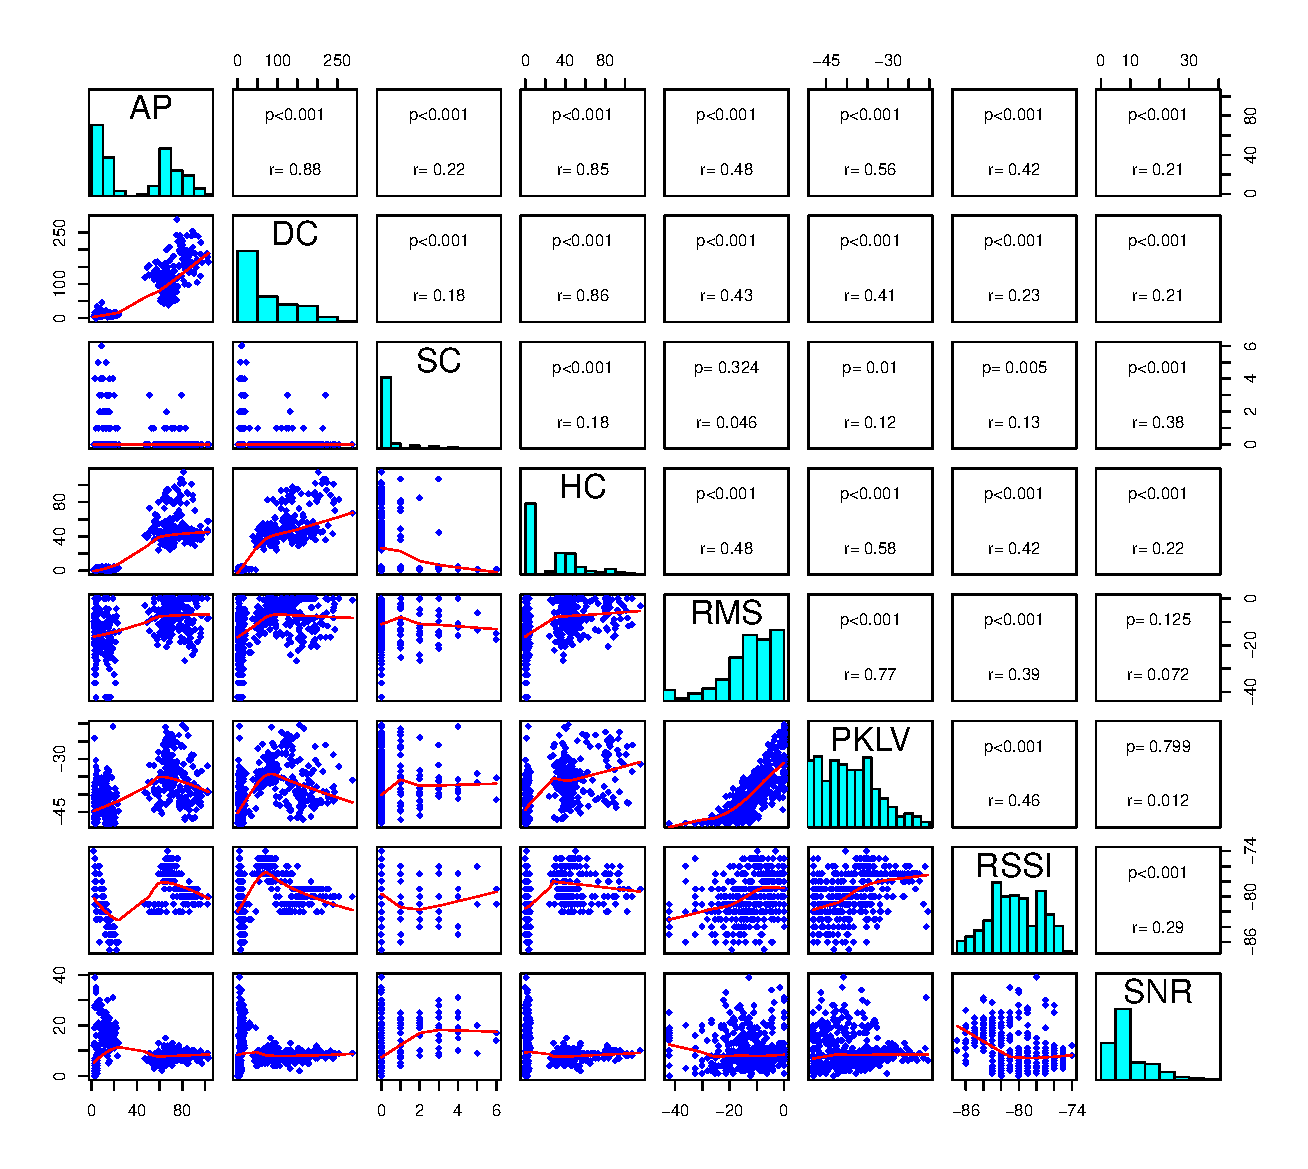
\includegraphics[width=1.3\textwidth]{./img/result/all-result}
		\end{adjustwidth}
		\caption[Scatter plot matrix of all parameters.]
		{Scatter plot matrix showing all parameters correlation of all collected data. The top right shows the correlation coefficient $r$ and the p-value. Along the diagonal are the histograms of each parameter.}
		\label{fig:scatterplot-matrix}
	\end{figure}

	% In the next chapter, we present regression analysis about social level density estimation using all data from four days experiment. The regression analysis tries to estimate the social density estimation using consumer smartphone sensor readings.

	% We predict the head count or device count from other parameters, e.g., \ac{AP}, \ac{RMS}, \ac{PKLV}, and \ac{RSSI}. We do not use \ac{SC} as a predicting variable because speaker count value is almost at zero, which does not give us any meaningful insight, and we do not use \ac{SNR} parameter as well, because we derive signal to noise ratio from probe request packet capture in a laptop, which smartphone cannot capture.

	% Make the datasets available online.
	% Make sure that the data is available publicly, mention the url.

% regression
% \added{
\section{Social Density Prediction} % (fold)
\label{sec:social-density-prediction}
We construct data models so that we are able to predict the level of social density from new data. We use supervised learning techniques using three predictors, namely linear regression, k-Nearest Neighbor (\ac{k-NN}), and Support Vector Machine (\ac{SVM}), so that we can compare which predictor gives optimal model.

We predict the head count or device count from other parameters, e.g., \ac{AP}, \ac{RMS}, \ac{PKLV}, and \ac{RSSI}. We do not use \ac{SC} as a predicting variable because speaker count value is almost at zero, which does not give us any meaningful insight, and we do not use \ac{SNR} parameter as well, because we derive signal to noise ratio from probe request packet capture in a laptop, which smartphone cannot capture. Our dataset contains 459 records.

We validate our model using 10-folds cross-validation, which is a method to assess the performance of a prediction model. The cross-validation technique involves dataset partition into complementary subsets, namely training and testing sets, in which training subsets are for performing the analysis, while testing subsets are for the validation of the resulting model. 10-folds cross-validation divides the dataset to 10 complementary subsets, in which one subset will be the testing set and the other nine subsets are the training set, interchangeably in 10 times.
% }

We use \ac{RMSE} as the metric for cross-validation. In this metric, the optimal model has lower \ac{RMSE} value. The formula of \ac{RMSE} is as follows,
\begin{equation} \label{eq:rmse}
 RMSE=\sqrt { \frac { \sum _{ i=1 }^{ n }{ { \left( { p }_{ i }-{ a }_{ i } \right)  }^{ 2 } }  }{ n }  } 
\end{equation}
where ${ p }_{ i }$ is the predicted value, ${ a }_{ i }$ is the actual value, and $n$ is the number of cases. We implement the analysis using R~\cite{r-team}, presented in \autoref{ch:R-code-listings}.


	\subsection{Linear Regression} % (fold)
	\label{sub:linear_estimator}
	Linear regression is a method of modeling the relationship between a dependent variable and an explanatory (or predicting) variable by fitting a straight line across the data. A condition where there is only one explanatory variable is called simple linear regression, while multiple linear regression involves more than one explanatory variable. The result of linear regression is a linear function (or a model) with the explanatory variables as the parameters.

	To obtain a model with minimal error, we perform an exhaustive search for the best subsets of the predictors for predicting the dependent variable (head or device count) in linear regression. We use \ac{RMSE} of 10-folds cross-validation to select the optimal model using the smallest value. \autoref{r-code-linear-regr}~displays the implementation of linear regression analysis. We implement linear regression in R using \verb|caret| library~\cite{caret}. 
	
	\begin{figure}[H]
		\begin{adjustwidth}{-1cm}{}
		\centering
		\subfloat[head count]{
			\label{fig:tuning-linear-headcount}{
				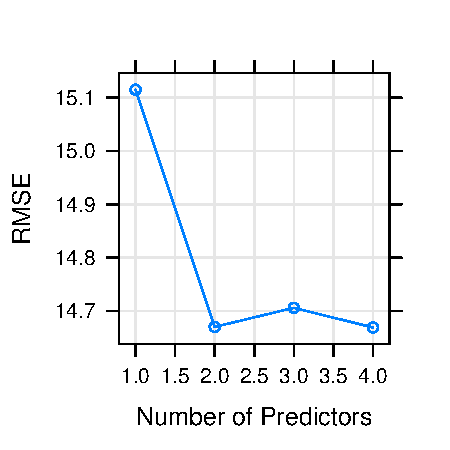
\includegraphics[width=0.65\textwidth]{./img/modeling/linear-regr-hc-small}
			}
		}
		\subfloat[device count]{
			\label{fig:tuning-linear-devicecount}{
				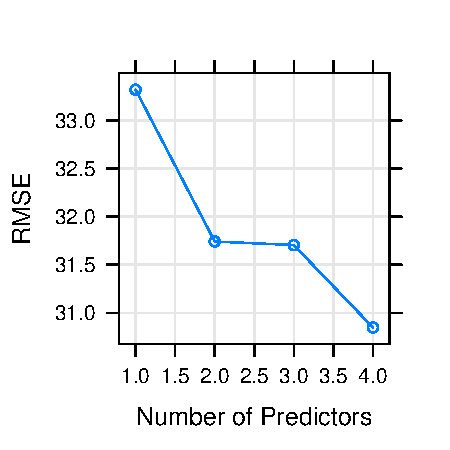
\includegraphics[width=0.65\textwidth]{./img/modeling/linear-regr-dc-small}
			}
		}
		\end{adjustwidth}
		\caption[Tuning linear regression.]
		{Tuning linear regression using best subsets combination for head count (\ref{fig:tuning-linear-headcount}) and device count (\ref{fig:tuning-linear-devicecount}). The result indicates that using all predictors gives the best result, although in head count prediction using two predictors results in nearly the same error.}
		\label{fig:tuning-linear}
	\end{figure}

	\autoref{fig:tuning-linear}~presents the tuning result. For both head count and device count, using all four predictors results in optimal model. In head count prediction, using two predictors ($ap$ and $pklv$) yields in nearly identical \ac{RMSE} as using four predictors. Based on the tuning, we develop a linear model to predict the head count and device count. The linear regression fit to the dataset is depicted in~\autoref{tab:linear-model-hc-dc}.

	
		\begin{table}[h]
		\centering
		\caption[Linear model fit to the dataset]
		{Linear model fit to the dataset with corresponding coefficient for head count and device count model.}
		\label{tab:linear-model-hc-dc}
		\begin{tabular}{rrr}
		\toprule
		\multicolumn{1}{l}{\multirow{2}{*}{Term}} & \multicolumn{2}{c}{Coefficient}                                   \\
		\multicolumn{1}{l}{}                      & \multicolumn{1}{c}{Head count} & \multicolumn{1}{c}{Device count} \\ \midrule
		\verb|Intercept|                          & 54.675 & -367.901 \\
		\verb|ap|                                 & 0.653  & 2.021 \\
		\verb|rms|                                & -0.109 & 1.138 \\
		\verb|pklv|                               & 0.760  & -1.880 \\
		\verb|rssi|                               & 0.329  & -3.656 \\ \bottomrule
		\end{tabular}
		\end{table}
	

	% , using an efficient branch-and-bound algorithm. 

	% predictions and real result, show the graph as well, better using line graph
	% mention what is the training and what is the testing (better using 10 fold cross validation)
	

	% hc ==========================
	% Subset selection object
	% 4 Variables  (and intercept)
	%      Forced in Forced out
	% ap       FALSE      FALSE
	% rms      FALSE      FALSE
	% pklv     FALSE      FALSE
	% rssi     FALSE      FALSE
	% 1 subsets of each size up to 4
	% Selection Algorithm: forward
	%          ap  rms pklv rssi
	% 1  ( 1 ) "*" " " " "  " " 
	% 2  ( 1 ) "*" " " "*"  " " 
	% 3  ( 1 ) "*" " " "*"  "*" 
	% 4  ( 1 ) "*" "*" "*"  "*" 

	% Linear Regression with Stepwise Selection 

	% 459 samples
	%   4 predictor

	% No pre-processing
	% Resampling: Cross-Validated (10 fold, repeated 10 times) 
	% Summary of sample sizes: 414, 413, 412, 412, 412, 413, ... 
	% Resampling results across tuning parameters:

	%   nvmax  RMSE      Rsquared 
	%   1      15.11505  0.7320710
	%   2      14.67019  0.7467084
	%   3      14.70598  0.7455704
	%   4      14.66907  0.7467488

	% RMSE was used to select the optimal model using  the smallest value.
	% The final value used for the model was nvmax = 4. 

	% Call:
	% lm(formula = gt ~ ., data = phone_data_gt)

	% Coefficients:
	% (Intercept)           ap          rms         pklv         rssi  
	%     54.6750       0.6530      -0.1091       0.7603       0.3288 

	% \begin{figure}[h]
	% 	\centering
	% 	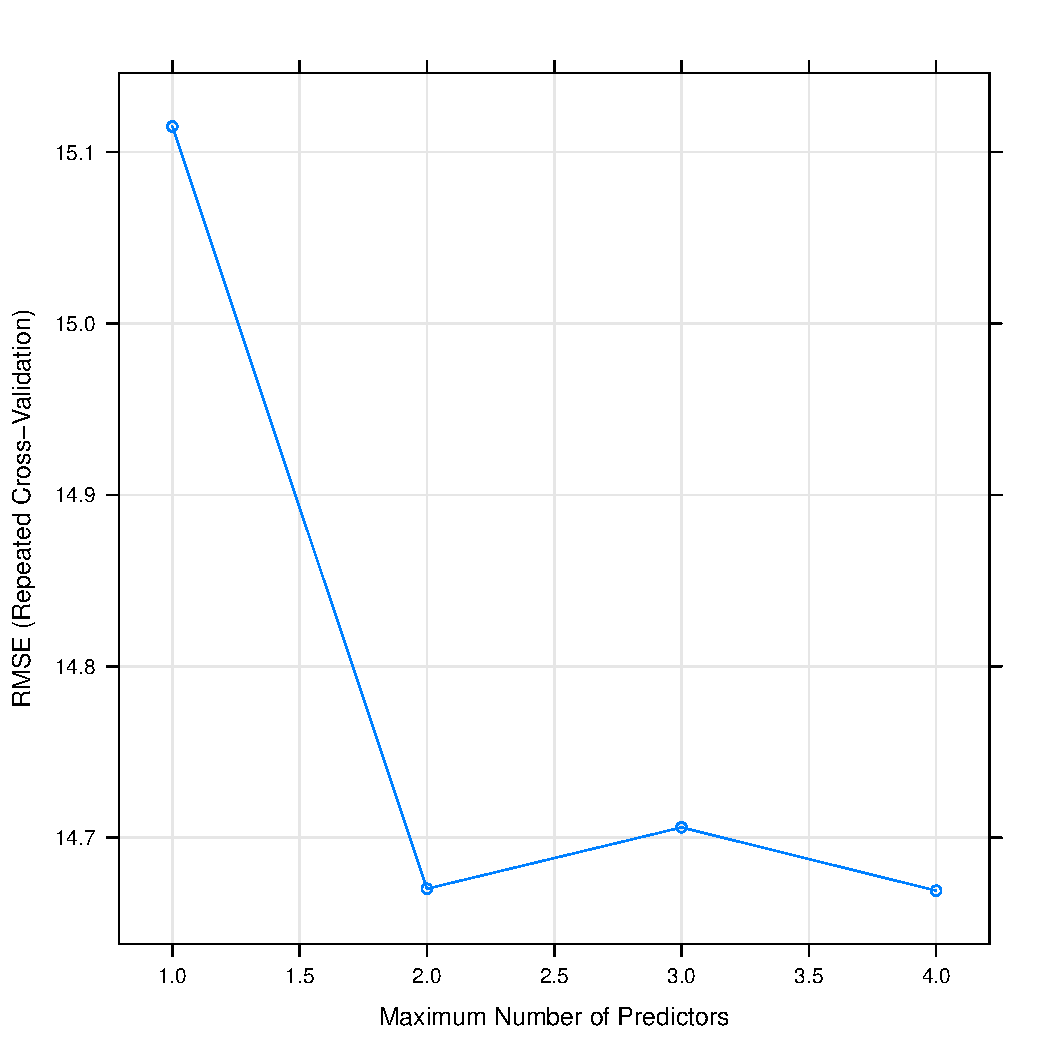
\includegraphics[width=0.9\textwidth]{./img/modeling/linear-regr-hc}
	% 	\caption{Tuning for linear regression.}
	% 	\label{fig:tuning-linear-hc}
	% \end{figure}

	% dc =========================
	% Subset selection object
	% 4 Variables  (and intercept)
	%      Forced in Forced out
	% ap       FALSE      FALSE
	% rms      FALSE      FALSE
	% pklv     FALSE      FALSE
	% rssi     FALSE      FALSE
	% 1 subsets of each size up to 4
	% Selection Algorithm: 'sequential replacement'
	%          ap  rms pklv rssi
	% 1  ( 1 ) "*" " " " "  " " 
	% 2  ( 1 ) "*" " " " "  "*" 
	% 3  ( 1 ) "*" " " "*"  "*" 
	% 4  ( 1 ) "*" "*" "*"  "*" 

	% Linear Regression with Stepwise Selection 

	% 459 samples
	%   4 predictor

	% No pre-processing
	% Resampling: Cross-Validated (10 fold, repeated 10 times) 
	% Summary of sample sizes: 414, 414, 413, 411, 414, 413, ... 
	% Resampling results across tuning parameters:

	%   nvmax  RMSE      Rsquared 
	%   1      33.32081  0.7752300
	%   2      31.74120  0.7979257
	%   3      31.70418  0.7990889
	%   4      30.84697  0.8103420

	% RMSE was used to select the optimal model using  the smallest value.
	% The final value used for the model was nvmax = 4.

	% Call:
	% lm(formula = pr ~ ., data = phone_data_pr)

	% Coefficients:
	% (Intercept)           ap          rms         pklv         rssi  
	%    -367.901        2.021        1.138       -1.880       -3.656 
	% \begin{figure}[h]
	% 	\centering
	% 	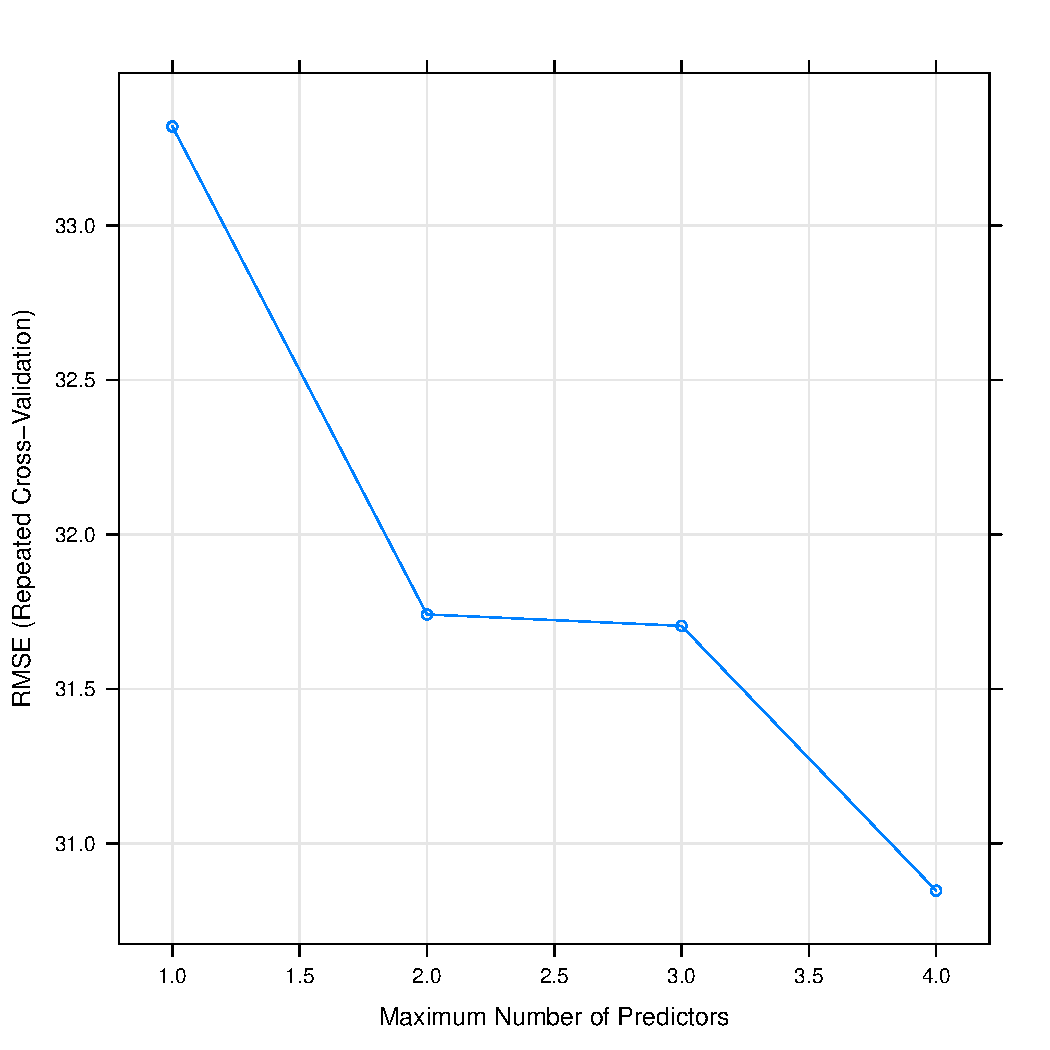
\includegraphics[width=0.9\textwidth]{./img/modeling/linear-regr-dc}
	% 	\caption{Tuning for linear regression.}
	% 	\label{fig:tuning-linear-dc}
	% \end{figure}

	\subsection{k-Nearest Neighbor} % (fold)
	\label{sub:k_nearest_neighbor}
	% subsection k_nearest_neighbor (end)
	% =====================knn===================================
	k-Nearest Neighbor (\ac{k-NN}) is an algorithm that predicts numerical value based on similarity measure using distance function of k-nearest neighbors of the predicted value.
	% Generally, a large $k$ value is more accurate as it uses more neighbors to predict a new value. \ac{k-NN} is applicable for both classification and regression analysis.

	\begin{figure}[H]
		\begin{adjustwidth}{-1cm}{}
		\centering
		\subfloat[head count]{
			\label{fig:tuning-knn-hc}{
				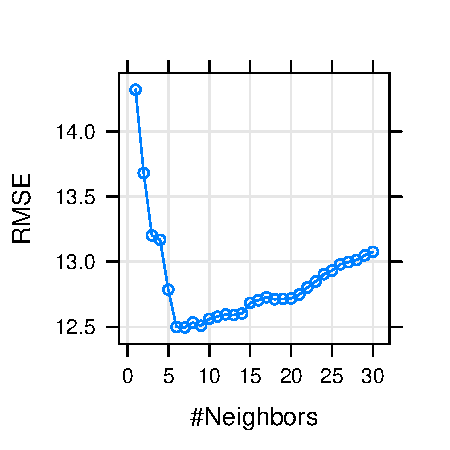
\includegraphics[width=0.65\textwidth]{./img/modeling/knn-hc-small}
			}
		}
		\subfloat[device count]{
			\label{fig:tuning-knn-dc}{
				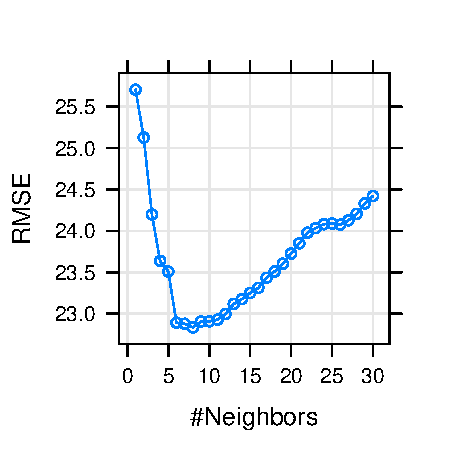
\includegraphics[width=0.65\textwidth]{./img/modeling/knn-dc-small}
			}
		}
		\end{adjustwidth}
		\caption[Tuning \ac{k-NN}.]
		{Tuning \ac{k-NN} using $1 \le k \le 30$ as the tuning parameter (\#Neighbors) for head count (\ref{fig:tuning-knn-hc}) and device count (\ref{fig:tuning-knn-dc}). For both estimation, optimal result is obtained when $5 \le k \le 10$. The optimal result is chosen at $k=7$ (head count) and $k=8$ (device count).}
		\label{fig:tuning-knn}
	\end{figure}

	We train and test \ac{k-NN} regression using $1 \le k \le 30$ as the tuning parameter in R using \verb|caret| library~\cite{caret}. Similar in the linear regression analysis, we evaluate the model using 10-folds cross-validation and we use \ac{RMSE} to select the optimal model with lowest error. \autoref{r-code-knn}~displays the implementation of \ac{k-NN} regression.

	\autoref{fig:tuning-knn}~presents the tuning result.
	% As we can see, the optimal models are obtained when $5 \le k \le 10$.
	According to~\autoref{fig:tuning-knn}, the highest error of both estimation is when $k=1$ and there is an increasing trend of error as $k$ goes up.
	% \added{
		The tuning results indicate that the optimal model for head count estimation is achieved when $k=7$ ($RMSE=12.49515$), while the optimal model for device count estimation is when $k=8$ ($RMSE=22.83321$).
	% }
	% hc ========================================================
	% k-Nearest Neighbors 

	% 459 samples
	%   4 predictor

	% No pre-processing
	% Resampling: Cross-Validated (10 fold, repeated 10 times) 
	% Summary of sample sizes: 414, 413, 412, 412, 412, 413, ... 
	% Resampling results across tuning parameters:

	%   k   RMSE      Rsquared 
	%    1  14.32195  0.7651252
	%    2  13.68100  0.7813994
	%    3  13.20218  0.7946098
	%    4  13.16852  0.7956532
	%    5  12.78561  0.8064473
	%    6  12.49908  0.8149187
	%    7  12.49515  0.8156143
	%    8  12.53433  0.8148571
	%    9  12.50869  0.8159582
	%    ...
	%   30  13.07611  0.7998607

	% RMSE was used to select the optimal model using  the smallest value.
	% The final value used for the model was k = 7. 

	%             Length Class      Mode     
	% learn       2      -none-     list     
	% k           1      -none-     numeric  
	% theDots     0      -none-     list     
	% xNames      4      -none-     character
	% problemType 1      -none-     character
	% tuneValue   1      data.frame list     
	% obsLevels   1      -none-     logical  

	% dc ========================================================
	% k-Nearest Neighbors 

	% 459 samples
	%   4 predictor

	% No pre-processing
	% Resampling: Cross-Validated (10 fold, repeated 10 times) 
	% Summary of sample sizes: 414, 414, 413, 411, 414, 413, ... 
	% Resampling results across tuning parameters:

	%   k   RMSE      Rsquared 
	%    1  25.70729  0.8686436
	%    2  25.12761  0.8746131
	%    3  24.19895  0.8823375
	%    4  23.63810  0.8880587
	%    5  23.50962  0.8894205
	%    6  22.89128  0.8950484
	%    7  22.87820  0.8953308
	%    8  22.83321  0.8958578
	%    9  22.90468  0.8955070
	%   10  22.90716  0.8953828
	%   ...
	%   30  24.42160  0.8851021

	% RMSE was used to select the optimal model using  the smallest value.
	% The final value used for the model was k = 8. 

	%             Length Class      Mode     
	% learn       2      -none-     list     
	% k           1      -none-     numeric  
	% theDots     0      -none-     list     
	% xNames      4      -none-     character
	% problemType 1      -none-     character
	% tuneValue   1      data.frame list     
	% obsLevels   1      -none-     logical 


	\subsection{Support Vector Machine} % (fold)
	\label{sub:support_vector_machine}
	% subsection support_vector_machine (end)
	% =======================svm=============================================
	Support Vector Machine (\ac{SVM}) is an estimator that works by constructing support vectors (hyperplanes) that separate the data according to a certain threshold. Most of the time, a kernel, a set of mathematical functions, is used to
	define the decision boundary.
	% \ac{SVM} is also implementable for both classification and regression analysis.

	We implement \ac{SVM} to predict quantities using radial kernel with $cost$ and $\epsilon$ as the tuning parameters.
	$cost$ parameter is used to define the width of the hyperplane, while $\epsilon$ is used to determine how non-linear the decision boundary is.
	As used in \ac{k-NN}, we validate the model using 10-folds cross-validation.
	We use grid search method to tune the optimal parameters. It tries to find the best combination of the two parameters in certain range of search.
	We implement the analysis in R with \verb|e1071| library~\cite{e1071}. \autoref{r-code-svm}~displays the implementation of \ac{SVM} prediction.

	\begin{figure}[H]
		\begin{adjustwidth}{-3cm}{}
		\centering
		\subfloat[head count]{
			\label{fig:tuning-svm-hc}{
				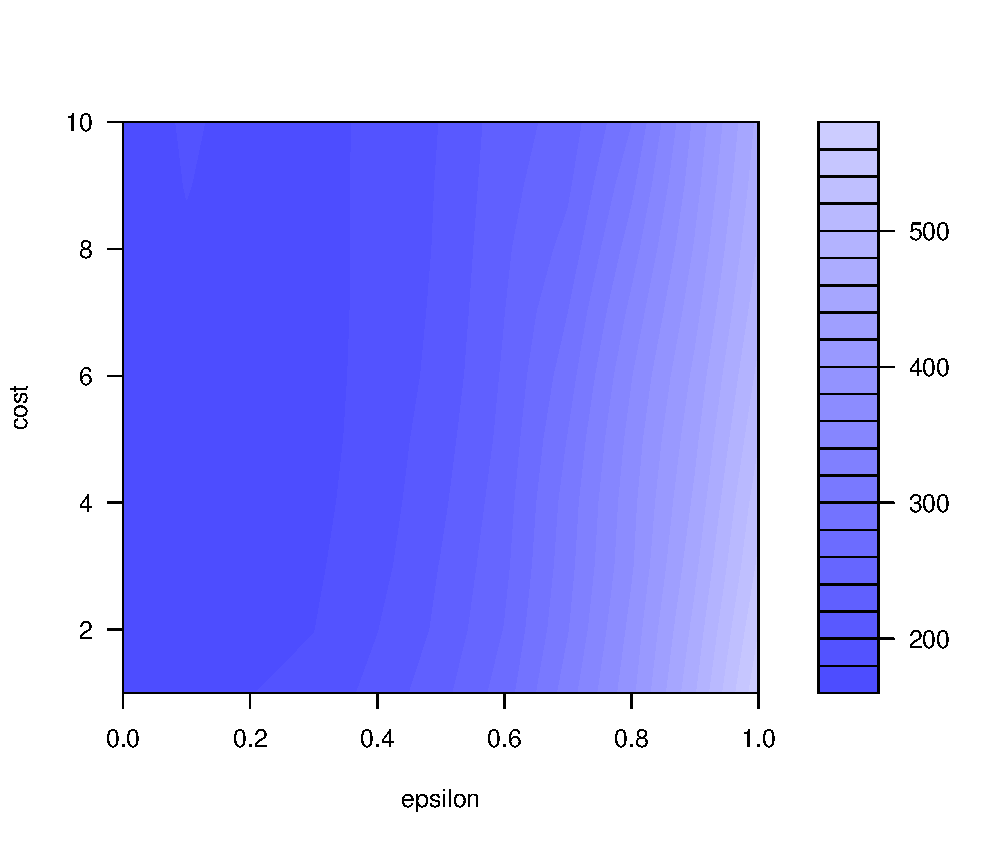
\includegraphics[width=0.65\textwidth]{./img/modeling/svm-hc}
			}
		}
		\subfloat[device count]{
			\label{fig:tuning-svm-dc}{
				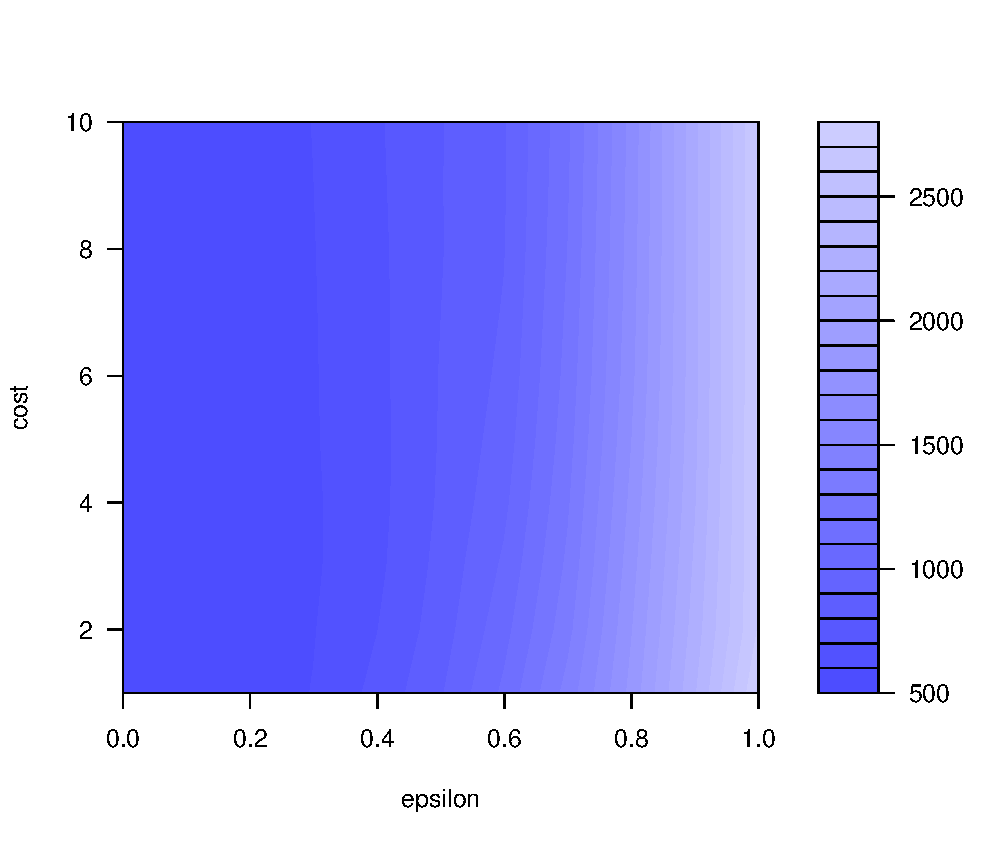
\includegraphics[width=0.65\textwidth]{./img/modeling/svm-dc}
			}
		}
		\end{adjustwidth}
		\caption[Tuning \ac{SVM}.]
		{Tuning \ac{SVM} using grid search technique. Two tuning parameters $\epsilon$ and $cost$ are represented in $x$ and $y$ axis, while the performance (measured using \ac{MSE}) is represented in color. More optimal model is indicated by darker color, i.e., lower \ac{MSE} (see color bar).}
		\label{fig:tuning-svm}
	\end{figure}

	We present the result of \ac{SVM} regression tuning in~\autoref{fig:tuning-svm}.
	% \added{
	We focus the grid search within $0 \le cost \le 10$ and $0 \le \epsilon \le 1$ to reduce the computational time. Moreover, our previous grid search, which involves wider area, indicates that \ac{SVM} performs better within that area.
	% }

	We measure the performance of the \ac{SVM} using mean squared error (\ac{MSE}), in which best result has lower \ac{MSE}. The best performance for head count prediction is at 171.1065 with $\epsilon=0$ and $cost=3$, while for device count prediction is at 514.226 with $\epsilon=0$ and $cost=1$. We can also see a trend of increasing \ac{MSE} as the $epsilon$ increases.
	% hc============
	% Parameter tuning of 'svm':

	% - sampling method: 10-folds cross validation 

	% - best parameters:
	%  epsilon cost
	%        0    3

	% - best performance: 171.1065 


	% dc============
	% Parameter tuning of 'svm':

	% - sampling method: 10-folds cross validation 

	% - best parameters:
	%  epsilon cost
	%        0    1

	% - best performance: 514.226 

To summarize the regression analysis and to interpret the result, we use another approach to calculate the error, which has more intuitive interpretation. We use residual error, which can be formulated as

\begin{equation}\label{eq:residual-error}
	\overline { error } =\frac { 1 }{ n } \left( \sum _{ i=1 }^{ n }{ \left| { p }_{ i }-{ a }_{ i } \right|  }  \right) 
\end{equation}

\noindent
As formulated in the equation, residual error shows the mean of the difference between predicted and actual value. Using the optimum model of each regression technique, we perform another 10-fold cross validation to obtain residual error measurement. The optimal model has a residual error closer to zero.

\begin{table}[h]
\centering
\caption[Summary of regression analysis]
{Summary of regression analysis showing the range of the data and the residual error of each regression method.}
\label{tab:regression-summary}
\begin{tabular}{llllll}
\toprule
                   & \multicolumn{2}{c}{Value Range}                         & \multicolumn{3}{c}{Residual Error}                                                        \\
                   & \multicolumn{1}{c}{Min} & \multicolumn{1}{c}{Max} & \multicolumn{1}{c}{Linear} & \multicolumn{1}{c}{k-NN} & \multicolumn{1}{c}{SVM} \\ \midrule
Head count estimation   & 0                       & 115                     & 9.89                                  & 7.05                    & 7.06                    \\
Device count estimation & 0                       & 288                     & 23.81                                 & 13.14                   & 13.34                  \\ \bottomrule
\end{tabular}
\end{table}

\autoref{tab:regression-summary}~presents the summary of the regression analysis. \ac{k-NN} and \ac{SVM} have better performance than the linear regression. \ac{k-NN} and \ac{SVM} do not have much difference of error for both head count and device count estimation. Device count estimation has wider value range and error compared to head count estimation.

% Plot the prediction graph in each cross validation round, then combined.
% Explain the result in percentage as well, instead of manual count. -> for the error in the modeling.
% plot the graph of head count (real vs predicted) vs parameters (ap count, or anything else)
% present the evaluation in people count and also percentage

%*****************************************
%*****************************************
%*****************************************
%*****************************************
%*****************************************
